\documentclass{report}
\usepackage[utf8]{vietnam}
\usepackage[utf8]{inputenc}
\usepackage{amsmath}
\usepackage{amsfonts}
\usepackage{bbold}
\usepackage{bbm}
\usepackage{array}
\usepackage{tabu}
\usepackage[justification=centering]{caption}
\usepackage{amssymb}
\usepackage{axodraw4j}
\usepackage{color}
\usepackage{epsfig}
\usepackage{epstopdf}
\usepackage{graphicx}
\usepackage{multirow}
\usepackage[nodayofweek,level]{datetime}

%%%%%%%%%%%%%%%%%%%%%%
\setlength{\arrayrulewidth}{0.4mm}
\setlength{\tabcolsep}{18pt}
\renewcommand{\arraystretch}{1.5}
\newcommand{\mydate}{\formatdate{3}{6}{1994}}

\title{\textbf{Luận văn tốt nghiệp:\\Tổng hợp bài giảng về đại số Lie ứng dụng trong lý thuyết hạt cơ bản}} 
\author{Nguyễn Quốc Chương}

\begin{document}

\pagenumbering{gobble}

\begin{titlepage}
		\maketitle
\end{titlepage}

\tableofcontents

\setcounter{page}{1}
\pagenumbering{arabic}

\chapter{EXPONENTIAL CỦA MA TRẬN}

\section{Chuẩn của ma trận: norm}
	
Cho A là ma trận cấp n, A = \((a_{ij}) \), \(a_{ij} \in \mathbb{F} \), ta định nghĩa chuẩn của ma trận như sau:

\[ ||A|| = \sqrt{ \sum_{i, j=1}^n |a_{ij}|^{2} } \]

Ta kí hiệu \( A = (a_{ij}) \leftrightarrow ( a_{11}, a_{12}, ..., a_{1n}, ..., a_{n1}, ..., a_{nn} ) \) 

||A|| còn được gọi là tích Descartes do tương ứng với một module của vector trong không gian euclid \( F^{n^{2}} \)\\

\textbf{\underline{Mệnh đề:}}

	\begin{enumerate}
 		\item \( ||A|| \geq 0, ||A|| = 0 \Leftrightarrow A = 0_{n \times n} \)
 		\item \( ||\alpha A|| = |\alpha |.||A||, \alpha \in \mathbb{C} \)
 		\item \( ||AB|| \leq ||A||.||B|| \)
 		\item \( ||A + B|| \leq ||A|| + ||B|| \)
	\end{enumerate}

Dãy ma trận \( A_{k} \) hội tụ về ma trận A nếu \( \forall \varepsilon \textgreater 0, \exists N_{ \varepsilon } \textgreater 0 \) sao cho \( || A_{k} - A || \textless \varepsilon \) với \( k \textgreater N_{ \varepsilon}\);  \(k, N_{\varepsilon} \) nguyên dương.\\

Kí hiệu: \[ \lim_{k \to \infty} A_{k} = A \] 

\underline{Bài tập:} Đặt dãy \( A_{k} = (a_{k,ij}) \) và \( A = (a_{ij}) \), với \( i,j = \overline{1,n} \). Chứng minh \( \lim_{k \to \infty} A_{k} = A \) khi và chỉ khi \( \lim_{k \to \infty} a_{k,ij} = a_{ij} \).\\

Dãy ma trận \(A_{k} \) là dãy Cauchy nếu  \( \forall \varepsilon \textgreater 0, \exists N_{ \varepsilon } \textgreater 0 \): \( || A_{m} - A_{k} || \textless \varepsilon\) \( \forall k, m \textgreater N_{ \varepsilon} \).\\

\underline{Bài tập:} Chứng minh nếu dãy ma trận \( A_{k} \) là dãy cauchy thì tồn tại \( \lim_{k \to \infty} A_{k} = A \) và ngược lại.

\section{Hàm exp}

A là ma trận cấp n, ta có hàm exp của ma trận A như sau:

	\[ e^{A} = \sum_{j=0}^{ \infty } \frac{A^{j}}{j!} = \mathbb{I}_{n} + A + \frac{A^{2}}{2!} + \dots \]
	
Hàm exp tồn tại cho mọi ma trận A. ta quy ước \(A^{0} = \mathbb{I}_{n} \)

\underline{Bài tập:} xét dãy tổng riêng phần sau:

	\[S_{m} = \sum_{j=0}^{ \infty } \frac{A^{j}}{j!} \]

chứng minh \( S_{m} \) là dãy Cauchy.\\

\textbf{\underline{Mệnh đề:}} cho \( A \in L(n) \)

	\begin{enumerate}
		\item \( e^{\mathbb{O}} = \mathbb{I}_{n} \) với \( \mathbb{O} \) là ma trận 0
		\item nếu \( AB = BA \) thì \( e^{A+B} = e^{A}e^{B} = e^{B}e^{A} \)
		\item \( (e^{A})^{-1} = e^{-A} \) với \( e^{A} \in GL(n) \) 
		\item nếu ma trận B khả nghịch thì \( Be^{A}B^{-1} = e^{BAB^{-1}} \)
		\item det(\( e^{A} \)) = \( e^{Tr(A)} \)
		\item \( (e^{A})^{T} = e^{A^{T}} \), tương tự cho \( (e^{A})^{\dagger} = e^{A^{\dagger}} \)
		\item  \( \frac{d}{dt}(e^{tA}) = Ae^{tA} = e^{tA}A \) với t là số thực
	\end{enumerate}
	
\underline{Bài tập:} Chứng minh các mệnh đề trên.\\	

\section{Đạo hàm của ma trận}

Cho \( A(t) = (a_{ij}(t)) \in L(n) \) với \( t \in \mathbb{R} \), ta có đạo hàm của ma trận như sau:

\[ \frac{d}{dt}(A(t)) = \lim_{ h \to \infty } \frac{A(t+h) - A(t)}{h} \]

\underline{Bài tập:} Chứng minh

\[ \frac{d}{dt}(A(t)) = (\frac{d}{dt}(a_{ij}(t)) \] 
\[ \frac{d}{dt}(A(t)B(t)) = \frac{d}{dt}(A(t))B(t) + B(t)\frac{d}{dt}(B(t)) \]
\[ \frac{d}{dt}(A(t) + B(t)) = \frac{d}{dt}(A(t)) + \frac{d}{dt}(B(t)) \]

\section{Logarithm của một ma trận}

Ta có các tính chất sau:

\[ ln(B) = \sum_{j=1}^{ \infty } \frac{(-1)^{j+1}}{j}(B - \mathbb{I})^j, ||B - \mathbb{I}|| \textless 1 \]
\[ e^{lnB} = B, ||B - \mathbb{I}|| \textless 1 \]
\[ ln(e^{A}) = A, ||e^{A} - \mathbb{I}|| \textless 1 \]

\textbf{\underline{Mệnh đề:}}

Với M(n) là tập các ma trận cấp n (không đòi hỏi tính khả nghịch) và GL(n) là tập các ma trận cấp n khả nghịch, ta có các mệnh đề sau:

	\begin{enumerate}
		\item \( \forall \varepsilon \textgreater 0 \), \( \exists \delta \textgreater 0 \) sao cho \( ||A|| \textless \delta \Rightarrow || e^{A} - \mathbb{I} || \textless \varepsilon \).\\ \textbf{Đặc biệt:} \( ||A|| \textless ln2 \Rightarrow ||e^{A} - \mathbb{I} || \textless 1 \)
		\item Tồn tại lân cận mở \( V \subset M(n) \), \( \mathbb{O} \in V \) và quả cầu mở \( B_{\varepsilon}(\mathbb{I}) \subset GL(n) \) sao cho ánh xạ exp: \( V \rightarrow B_{\varepsilon}(\mathbb{I}) \) là song ánh.
	\end{enumerate}

\underline{Bài tập:} Chứng minh các mệnh đề trên

\textbf{Chú ý:} Với mỗi ma trận B trong lân cận của ma trận đơn vị \( \mathbb{I} \), tồn tại duy nhất một ma trận A trong lân cận của ma trận \( \mathbb{O} \) sao cho \( e^{A} = B \) (điều này được áp dụng trong các bài học sau) và các phần tử của ma trận B là hàm giải tích của các phần tử ma trận A.

\chapter{NHÓM LIE MA TRẬN VÀ ĐẠI SỐ LIE}

Nhóm Lie ma trận (tuyến tính) là các nhóm con của \( GL(n,\mathbb{C}) \)

\section{Ma trận tiếp xúc và đường cong giải tích}

Cho G là nhóm Lie ma trận

A(t) là một đường cong giải tích trong G đi qua ma trận đơn vị \( \mathbb{I}_{n} \) sao cho:

	\begin{itemize}
		\item \( A(t) \subset G \) với \( t \subset \mathbb{R} \)
		\item \( A(0) = \mathbb{I}_{n} \)
		\item \( A(t) = (a_{ij}(t)) \), \(a_{ij}(t) \) là các hàm giải tích.
	\end{itemize}

Khi đó ma trận tiếp xúc với A(t) tại \( \mathbb{I}_{n} \) được định nghĩa như sau:

\[ \mathcal{A} = \left. {\frac{d}{dt}} \right|_{t=0} A(t) = \dot{A}(0) \] 

với \( \mathcal{A} \in  M(n,\mathbb{C}) \) 

\underline{Bài tập:} Chứng tỏ tập hợp các ma trận tiếp xúc có cấu trúc của một không gian tuyến tính ( gọi là g). 

\section{Giao hoán tử của hai ma trận tiếp xúc}

Giả sử ta có \( \mathcal{A} = \left. {\frac{d}{dt}} \right|_{t=0} A(t) \), \( \mathcal{B} = \left. {\frac{d}{dt}} \right|_{t=0} B(t) \)

ta định nghĩa giao toán tử như sau:

\[ [\mathcal{A}, \mathcal{B}] = \left. {\frac{d}{dt}} \right|_{t=0} (A(\tau)B(\tau)A^{-1}(\tau)B^{-1}(\tau)) \]

Trong đó \( t = \tau^{2} \) và \( A(\tau)B(\tau)A^{-1}(\tau)B^{-1}(\tau) \) là một đường cong giải tích trong G. Từ đó suy ra \( [\mathcal{A}, \mathcal{B}] \) là ma trận tiếp xúc của đường cong C(t) trong g với \( C(t) =  A(\tau)B(\tau)A^{-1}(\tau)B^{-1}(\tau) \).

Xét các khai triển Taylor sau:

\[ C(t) = \mathbb{I}_{n} + \varepsilon \tau + \dot{\varepsilon} \tau^{2} + \dots \]
\[ A(\tau) = \mathbb{I}_{n} + \mathcal{A} \tau + \dot{\mathcal{A}} \tau^{2} + \dots \]
\[ B(\tau) = \mathbb{I}_{n} + \mathcal{B} \tau + \dot{\mathcal{B}} \tau^{2} + \dots \]

Do \[ C(t)B(\tau)A(\tau) = A(\tau)B(\tau) \]
 
Suy ra \[ \mathbb{I}_{n} + ( \mathcal{A} + \mathcal{B} + \varepsilon ) \tau + ( \dot{\mathcal{A}} + \dot{\mathcal{B}} + \dot{\varepsilon} + \mathcal{B} \mathcal{A} +  \varepsilon \mathcal{B} + \varepsilon \mathcal{A} ) \tau^{2} + \dots = \mathbb{I}_{n} + ( \mathcal{A} + \mathcal{B} ) \tau + ( \dot{\mathcal{A}} + \dot{\mathcal{B}} + \mathcal{A} \mathcal{B} ) \tau^{2} + \dots \]
 
Tương đương 2 vế ta được: \( \varepsilon = 0 \), \( \dot{\varepsilon} = \mathcal{A} \mathcal{B} - \mathcal{B} \mathcal{A} \)

Mặt khác ta có: \( [\mathcal{A}, \mathcal{B}] = \left. {\frac{d}{dt}} \right|_{t=0} C(t) = \left. {\frac{d}{d \tau^{2}}} \right|_{\tau=0} ( \mathbb{I}_{n} + \dot{\varepsilon} \tau^{2} + \dots ) = \dot{\varepsilon} \)

Vậy \[ [\mathcal{A}, \mathcal{B}] = \mathcal{A} \mathcal{B} - \mathcal{B} \mathcal{A} \]

\textbf{Nhận xét:} 

\( \mathcal{A} \), \(\mathcal{B} \) phải là 2 ma trận tiếp xúc thì mới có biểu thức trên

Không gian các ma trận tiếp xúc g là đóng đối với các phép giao hoán tử do \( [\mathcal{A}, \mathcal{B}] \in \) g

\underline{Bài tập:} Chứng minh \( C(t) =  A(\tau)B(\tau)A^{-1}(\tau)B^{-1}(\tau) \)

\section{Đại số Lie}

Không gian tuyến tính L được trang bị phép nhân \( [X,Y] \in L \) được gọi là (cấu trúc) đại số Lie nếu thỏa các tính chất sau: 
 
	\begin{enumerate}
		\item \( [X,Y] = -[Y,X] \) (tính phản xứng)
		\item \( [[aX + bY],Z] = a[X,Z] + b[Y,Z] \) với \( a \), \( b \) \( \in \) \( \mathbb{C} \) (tính song tuyến tính)
		\item \( [[X,Y],Z] + [[Y,Z],X] + [Z,X],Y] = 0 \) (đẳng thức Jacobi)
	\end{enumerate}	 
 
\[ \forall X, Y, Z \in L \] 
 
Không gian các ma trận tiếp xúc g với phép nhân \( [\mathcal{A}, \mathcal{B}] = \mathcal{A} \mathcal{B} - \mathcal{B} \mathcal{A} \) được gọi là đại số Lie g của nhóm Lie G.

Nếu đại số Lie g có cơ sở \( \left\lbrace \mathcal{A}_{i}, i =1, 2, 3, ..., m \right\rbrace \) (với tư cách là không gian tuyến tính với dim(g) = m) thì rõ ràng:

\[ [\mathcal{A}_{i}, \mathcal{A}_{j}] = \sum_{k=1}^{m} c_{ijk}\mathcal{A}_{k} \]

Trong đó \( c_{ijk} \) còn được gọi là các hằng số cấu trúc của nhóm Lie G, ta có các tính chất sau:

	\begin{itemize}
		\item \( c_{ijk} = -c_{jik} \)
		\item \( c_{ijl}c_{lkm} + c_{jkl}c_{lim} + c_{kil}c_{ljm} = 0 \)
	\end{itemize}
 
\underline{Bài tập:}

1) Chứng minh các tính chất của các hằng số cấu trúc.

2) Chứng minh rằng nếu nhóm Lie G cũng giao hoán thì đại số Lie g cũng giao hoán, tức là \( [A,B] = 0 \Rightarrow [\mathcal{A}, \mathcal{B}] = 0 \)
  
\section{Phép tham số hóa các phần tử của nhóm Lie}  
Đầu tiên ta xét khái niêm nhóm con một tham số như sau:

Nhóm con một tham số của nhóm Lie G là một đường cong giải tích A(t) trong G sao cho:

	\begin{itemize}
	 \item \( A(s)A(t) = A(s+t) \) với |s|, |t| bé
	 \item \( A(0) = \mathbb{I}_{n} \)
	 \item \( \mathcal{A} = \dot{A}(0) \)
	\end{itemize}
	
\[ \Rightarrow \left. {\frac{d}{ds}} \right|_{s=0} A(t+s) = \left. {\frac{d}{ds}} \right|_{s=0} A(s)A(t) \]
\[ \Rightarrow \frac{d}{dt} A(t) = \mathcal{A}A(t) \]

Do |t| bé nên tồn tại nghiệm duy nhất \( A(t) = e^{t \mathcal{A} } \)

Như vậy ánh xạ exp: \[ g \rightarrow G \] có thể được xem như là \[ \mathcal{A} \rightarrow e^{\mathcal{A}} \]
		
Với t bé thì \(t\mathcal{A} \) gần với ma trận \( \mathbb{O} \), ánh xạ giải tích 1-1 và lên từ lân cận của \( \mathbb{O} \) trong g lên lân cận của phần tử đơn vị \( \mathbb{I}_{n} \) trong nhóm Lie G.

Nhắc lại: \( \left\lbrace \mathcal{A}_{i}, i = \overline{1,n} \right\rbrace \). Do đó mỗi phần tử trong g có dạng:

\[ \mathcal{A} = \sum_{i=1}^{m} \alpha_{i} \mathcal{A}_{i} \]

Suy ra mỗi phần tử của A trong lân cận đơn vị \( \mathbb{I}_{n} \) có dạng:


\[ A(\alpha) = exp \left( {\sum_{i=1}^{m} \alpha_{i} \mathcal{A}_{i}} \right) \] với \[ \alpha = (  \alpha_{1}, \alpha_{2}, ..., \alpha_{m} ) \]
	
\(	\alpha = (  \alpha_{1}, \alpha_{2}, ..., \alpha_{m} ) \) (có thể dùng để mô tả 1 phần tử trong nhóm lie G và \( \alpha \) phải đủ bé) là tọa độ chính tác của phần tử nhóm \( A(\alpha) \), m được gọi là số chiều của nhóm Lie G và được kí hiệu \( m = dim(G) \) ( m cũng chính là số tham số trong phép tham số hóa )

Như vậy ra đã dùng các tọa độ trong đại số Lie g để tham số hóa các phần tử của nhóm Lie G trong lân cận của ma trận đơn vị. 

Ta có:

\[ A(\alpha) = \mathbb{I}_{n} + \sum_{i=1}^{m} \alpha_{i} \mathcal{A}_{i} + \frac{1}{2} \sum_{i,k} \alpha_{i} \alpha_{k} \mathcal{A}_{i} \mathcal{A}_{k} + \dots \]

\textbf{Nhận xét:}

Các phần tử ma trận \( A(\alpha)_{pq} \) là các hàm giải tích theo tham số \( \alpha_{i} \), \( \overline{1,m} \), nên:

\[ \mathcal{A}_{i} = \left. \frac{\partial}{\partial \alpha_{i}} \right|_{\alpha = 0} A(\alpha) \]
\[ \alpha = 0 \Leftrightarrow (  \alpha_{1} = 0, \alpha_{2} = 0, ..., \alpha_{m} = 0) \]
\( \mathcal{A}_{i} \) còn được gọi là vi tử của đại số Lie g, để thuận tiện, ta viết lại:	

\[ A(\alpha) = e^{ i \left( { \alpha^{i} \mathcal{A}_{i}} \right) } \]
\[ \mathcal{A}_{i} = \frac{1}{i} \left. \frac{\partial A(\alpha)}{\partial \alpha^{i}} \right|_{\alpha = 0} \]

Trong đó i là số phức: \( i^{2} = -1 \)

\section{Nhóm Lie O(n), SO(n) và đại số Lie o(n), so(n)}

\[ O(n) = O(n,\mathbb{R}) = \left\lbrace A \in GL(n,\mathbb{R}: A^{T}A = \mathbb{I}_{n} \right\rbrace \]

Với \( A \in O(n) \) đủ gần với \( \mathbb{I}_{n} \), \( \exists ! \mathcal{A} \in M(n, \mathbb{R}) \) sao cho \( A = e^{\mathcal{A}} \)
	\begin{align*}
		& \Rightarrow (e^{\mathcal{A}})^T e^{\mathcal{A}} = \mathbb{I}_{n} \\
		& \Leftrightarrow (e^{\mathcal{A}})^T e^{\mathcal{A}} e^{\mathcal{-A}} = e^{\mathcal{-A}} \\
		& \Leftrightarrow (e^{\mathcal{A}})^T e^{\mathcal{A} - \mathcal{A}} = e^{\mathcal{-A}} \\
		& \Leftrightarrow (e^{\mathcal{A}})^T = e^{\mathcal{-A}} \\
		& \Leftrightarrow \mathcal{A}^T = \mathcal{-A}
	\end{align*}

Vậy đại số: \( o(n) = \left\lbrace { \mathcal{A} \in M(n,\mathbb{R}): \mathcal{A}^T = \mathcal{-A} } \right\rbrace \)

Nếu \( \mathcal{A}^T = \mathcal{-A} \)
\[ \Rightarrow Tr(\mathcal{A}) = 0 \Rightarrow det(A) = det(e^{\mathcal{A}}) = e^{Tr(\mathcal{A})} = e^{0} = 1 \]
\[ \Rightarrow A = e^{\mathcal{A}} \in SO(n)\]

Vậy \(so(n) = o(n) \)

\section{Nhóm Lie U(n), SU(n) và đại số Lie u(n), su(n)}

\[ U(n) = U(n,\mathbb{R}) = \left\lbrace A \in GL(n,\mathbb{R}: A^{\dagger}A = \mathbb{I}_{n} \right\rbrace \]

Với \( A \in U(n) \) đủ gần với \( \mathbb{I}_{n} \), \( \exists ! \mathcal{A} \in M(n, \mathbb{R}) \) sao cho \( A = e^{\mathcal{A}} \) \( \Rightarrow \mathcal{A}^{\dagger} = \mathcal{-A} \) với \( \mathcal{A} \) là toán tử phản Hermit.

Để tiện dụng, ta viết dưới dạng \( A = e^{ i \mathcal{A} } \Rightarrow e^{-i \mathcal{A}^{^{\dagger} }}e^{i \mathcal{A}} \Rightarrow \mathcal{A}^{\dagger} = \mathcal{A} \) với \( \mathcal{A} \) là toán tử Hermit.

Vậy đại số: \( u(n) = \left\lbrace { \mathcal{A} \in M(n,\mathbb{R}): \mathcal{A}^{\dagger} = \mathcal{A} } \right\rbrace \)

\textbf{Nhận xét:} Tập các ma trận hermit và phản hermit của đại số u(n) là như nhau: Nếu \( \mathcal{A} \) là phản hermit thì \( i \mathcal{A} \) là hetmit.

Nếu \( A \in SU(n) \): \( det(A) = det(e^{\mathcal{A}}) = e^{Tr(\mathcal{A})} = 1 \)

\[ \Rightarrow Tr(\mathcal{A}) = 0 \]

Vậy đại số Lie su(n) của SU(n) là:  \( su(n) = \left\lbrace { \mathcal{A} \in M(n,\mathbb{R}): \mathcal{A}^{\dagger} = \mathcal{A} }, Tr(\mathcal{A}) = 0 \right\rbrace \)

\underline{Bài tập:} Chứng minh số chiều của các đại số Lie như sau:

\[ dim (o(n)) = \frac{n(n-1)}{2} \]
\[ dim (u(n)) = n^{2} \]
\[ dim (su(n)) = n^{2} -1 \] 

\section{Nhóm quay SO(3) và đại số Lie so(3)}

Các phép quay trong \( \mathbb{R}^{3} \)

	\(R(\phi \vec{e}_{1}) \) = \( \begin{pmatrix}
	1 & 0 & 0 \\
	0 & cos(\phi) & sin(\phi) \\
	0 & -sin(\phi) & cos(\phi)
	\end{pmatrix} \) : quay quanh trục Ox
	
	\(R(\theta \vec{e}_{2}) \) = \( \begin{pmatrix}
	cos(\theta) & 0 & -sin(\theta) \\
	0 & 1 & 0 \\
	sin(\theta) & 0 & cos(\theta)
	\end{pmatrix} \) : quay quanh trục Oy
	
	\(R(\psi \vec{e}_{3}) \) = \( \begin{pmatrix}
	cos(\psi) & sin(\psi) & 0 \\
	-sin(\psi) & cos(\psi) & 0 \\
	0 & 0 & 1
	\end{pmatrix} \) : quay quanh trục Oz

Đặt: 

\(J_{1}\) = \( \frac{1}{i} \) \( \left. { \frac{ \partial R(\phi \vec{e}_{1}) }{\partial \phi} } \right|_{\phi = 0} \) = \( \begin{pmatrix}
	0 & 0 & 0 \\
	0 & 0 & -i \\
	0 & i & 0
	\end{pmatrix} \)
	
\[\]

\(J_{2}\) = \( \frac{1}{i} \) \( \left. { \frac{ \partial R(\theta \vec{e}_{2}) }{\partial \theta} } \right|_{\theta = 0} \) = \( \begin{pmatrix}
	0 & 0 & i \\
	0 & 0 & 0 \\
	-i & 0 & 0
	\end{pmatrix} \)	

\[\]

\(J_{3}\) = \( \frac{1}{i} \) \( \left. { \frac{ \partial R(\psi \vec{e}_{3}) }{\partial \psi} } \right|_{\psi = 0} \) = \( \begin{pmatrix}
	0 & -i & 0 \\
	i & 0 & 0 \\
	0 & 0 & 0
	\end{pmatrix} \)
	
\( \left\lbrace { J_{i} = 1, 2, 3 } \right\rbrace \) là cơ sở của đại số Lie so(3) với hệ thức giao hoán

\[ [J_{i}, J_{j}] = i \varepsilon_{ijk}J_{k} \]

trong đó  \( \varepsilon_{ijk} \) là tensor phản xứng hạng 3

Gọi \(\vec{\phi}\) = \( ( \vec{\phi}^{1}, \vec{\phi}^{2}, \vec{\phi}^{3} ) \in \mathbb{R}^{3} \) là vector xác định phép quay quanh trục quay \( \vec{n} = \frac{\vec{\phi}}{|\vec{\phi}|} \), với góc quay: \(\phi\) = \( |\vec{\phi}| \) = \( ( (\phi^{1})^{2} + (\phi^{2})^{2} + (\phi^{3})^{2} )^{1/2} \) 

\[ R(\vec{\phi}) = e^{i( \phi^{1} J_{1} + \phi^{2} J_{2} + \phi^{3} J_{3} )} = e^{i \vec{\phi} \vec{J}} = e^{i \phi \vec{n} \vec{J} } \]

\textbf{Nhận xét:} từ biểu thức trên ta có không gian tham số của so(3) là quả cầu mở có tâm tại (0,0,0): \( \left\lbrace { \vec{\phi} = ( \phi^{1}, \phi^{2}, \phi^{3}) \in \mathbb{R}^{3}, |\vec{\phi}| \textless 2 \pi }  \right\rbrace \)
	
\underline{Bài tập:} Tính \( e^{i \phi^{1} J_{1} }\), suy ra \( e^{i \phi^{1} J_{1}} \) = \( R(\phi \vec{e}_{1}) \)	

\section{Nhóm quay SU(2) và đại số Lie su(2) }
Ma trận \( \mathcal{A} \) cấp 2, hermitian và \(Tr(\mathcal{A}) = 0\) có thể được viết dưới dạng:
	
\( \mathcal{A} \) = \( \begin{pmatrix}
	\alpha^{3} & \alpha^{1} - i \alpha^{2} \\
	\alpha^{1} + i \alpha^{2} & - \alpha^{3} \\
	\end{pmatrix} \)  với \( \alpha^{1, 2, 3} \in \mathbb{R} \)

khai triển \( \mathcal{A} \) ta được:

\[ \mathcal{A} = \alpha^{1} \begin{pmatrix}
	0 & 1 \\
	1 & 0 \\
	\end{pmatrix} + \alpha^{2} \begin{pmatrix}
	0 & -i \\
	i & 0 \\
	\end{pmatrix} + \alpha^{3} \begin{pmatrix}
	1 & 0 \\
	0 & -1 \\
	\end{pmatrix} \]
	
Vậy các ma trận: \( \sigma_{1} \) = \( \begin{pmatrix}
	0 & 1 \\
	1 & 0 \\
	\end{pmatrix} \), \( \sigma_{2} \) = \( \begin{pmatrix}
	0 & -i \\
	i & 0 \\
	\end{pmatrix} \), \( \sigma_{3} \) = \(  \begin{pmatrix}
	1 & 0 \\
	0 & -1 \\
	\end{pmatrix} \) còn được gọi là các ma trận Pauli đồng thời cũng là cơ sở của đại số Lie su(2).
	
Ta đã biết: \( [\sigma_{i},\sigma_{j}] \) = \(2i \epsilon_{ijk} \sigma_{k} \)

Đặt phần tử sinh của su(2): \( J_{i}\) = \( \frac{\sigma_{i}}{2} \), i =1, 2, 3
	
Viết lại hệ thức giao hoán ta có: \( [J_{i},J_{j}] \) = \(i \epsilon_{ijk} J_{k} \) với \(J_{i}\) là ma trận thỏa mãn tính chất traceless và hermitian.

\underline{Bài tập:} chứng minh nếu \( U \in SU(2) \) thì U có thể viết được dưới dạng \( U \) = \(  \begin{pmatrix}
	\alpha & \beta \\
	\overline{-\beta} & \overline{\alpha} \\
	\end{pmatrix} \) trong đó \(\alpha\) = \( x_{1} + i x_{2} \), \(\beta\) = \( x_{3} + i x_{4} \) và \( x_{1, 2, 3, 4} \in \mathcal{R} \). Từ đó rút ra không gian tham số của SU(2) theo \( x_{1, 2, 3, 4} \) 
	
\section{Hằng số cấu trúc}

Đối với đại số Lie su(n) ta có biểu thức giao hoán: \([T_{i},T_{j}]=ic_{ijk}T_{k}\) với \(c_{ijk} \in \mathbb{R} \) và \(T_{i}^{\dagger}=T_{i}\)
	
Đặt \(\gamma_{ik} = Tr(T_{i}T_{k})\), ma trận \((\gamma_{ik})\) là đối xứng do	\(\gamma_{ik} = \gamma_{ki}\) 
	
	\begin{align*}
		\gamma_{ik}^{*} & = Tr(T_{i}^{*}T_{k}^{*}) \\
		& = Tr((T_{i}^{*}T_{k}^{*})^{T}) \\
		& = Tr((T_{k}^{*})^{T}(T_{i}^{*})^{T}) \\
		& = Tr(T_{k}^{\dagger}T_{i}^{\dagger}) \\
		& = Tr(T_{k}T_{i}) \\
		& = Tr(T_{i}T_{k}) \\
		& \Rightarrow \gamma_{ik}^{*} = \gamma_{ik}
	\end{align*}
	
ma trận \((\gamma_{ik})\) là ma trận thực đối xứng, nên có thể chéo hóa bằng ma trận trực giao (thực). Tức là tồn tại một ma trận trực giao

\[ R \gamma R^{-1} = diag(\lambda_{1},\lambda_{2},\dots,\lambda_{n})\]

với \( \lambda_{1},\dots,\lambda_{n} \) là các trị riêng của ma trận \(\gamma = (\gamma_{ik}) \) và \(R^{T} = R^{-1}\) 

	\begin{align*}
		\sum_{j,k} \gamma_{j,k} R_{ij} \gamma_{jk} R_{kl}^{-1} = \lambda_{i} \delta_{il} \\
		\Rightarrow \sum_{j,k} \gamma_{j,k} R_{ij} \gamma_{jk} R_{lk} = \lambda_{i} \delta_{il} 
	\end{align*}
	
Đặt: \(F_{i} = \sum_{j} R_{ij} T_{j}\), \(F_{i}^{\dagger} = F_{i} \)\\

Ta có: \(Tr(F_{i}F_{j}) = \sum_{j,k} R_{ij}R_{lk}Tr(T_{j}T_{k}) = \sum_{j,k}R_{ij}\gamma_{jk}R_{lk} = \lambda_{i}\delta_{il}\)\\

Ta chứng tỏ \(\lambda_{i} \textgreater 0 \) như sau:

	\begin{align*}
		\lambda_{i} & = Tr(F_{i}F_{i}) \\ 
		& = Tr(F_{i}F_{i}^{\dagger}) \\
		& = \sum_{\alpha,\beta} (F_{i})_{\alpha \beta} (F_{i})_{\alpha \beta}^{\dagger} \\
		& = \sum_{\alpha,\beta} \left| {(F_{i})_{\alpha \beta}} \right|^{2} \textgreater 0 \\
	\end{align*}
	
Đặt \(J_{i} = \sqrt{\frac{\lambda}{\lambda_{i}}} F_{i} \) \((\lambda \textgreater 0) \)	

	\begin{align*}
		\Rightarrow Tr(J_{i}J_{j}) & = \frac{\lambda}{\sqrt{\lambda_{i}\lambda_{j}}} Tr(F_{i}F_{j}) \\
		& =  \frac{\lambda}{\sqrt{\lambda_{i}\lambda_{j}}} \lambda_{i} \delta_{ij} \\
		& = \lambda \delta_{ij} \\
	\end{align*}
\[ Tr(J_{i}J_{j}) = \lambda \delta_{ij} \]

Ta có:
	\begin{align*}
		Tr([J_{i},J_{j}]J_{l}) & = ic_{ijk}Tr(J_{k}J_{l}) \\ 
		& = ic_{ijk} \lambda \delta_{kl} \\
		& = ic_{ijl} \lambda
	\end{align*}

\[ c_{ijl} = \frac{1}{i\lambda} Tr([J_{i}J_{j}]J_{l}) \]

\( \Rightarrow c_{ijl} \) là hoàn toàn phản xứng 

\chapter{CÁC PHÉP BIỂU DIỄN}

\section{Định nghĩa của phép biểu diễn}

Một biểu diễn của đại số Lie g là một đồng cấu R: \( g \longrightarrow GL(V) \) với \( GL(V) \) là tập các toán tử tuyến tính khả nghịch trong không gian vectơ V

	\[ \begin{matrix}
		 g & \longrightarrow & GL(V) \\
		 \downarrow & \hspace*{0cm} & \downarrow \\
		 X & \longrightarrow & R(X)
	\end{matrix} \]

\( R(X) \): toán tử tuyến tính trong không gian tuyến tính V (phức), khi đó dimV = n là số chiều của biểu diễn \( R \). Một biểu diễn thì có 2 tính chất sau

	\begin{itemize}
		\item \( R (aX + bY) = aR(X) + bR(Y) \): đồng cấu không gian vectơ
		\item \( R \left( \left[ X, Y \right] \right) = \left[ R(X), R(Y) \right] \): đồng cấu đại số
	\end{itemize}

Với \( \left[ R(X), R(Y) \right] = R(X)R(Y) - R(Y)R(X) \)\\

\underline{Ví dụ}: Đại số Lie su(2): \( \left[ T_{i}, T_{j} \right] = i \epsilon_{ijk} T_{k} \), \( T_{i} = \frac{\sigma_{i}}{2} \)

Biểu diễn cơ bản: \( R_{f}(T_{i}) = T_{i} \): ánh xạ cuyến tính từ không gian 2 chiều vào không gian 2 chiều \( \Rightarrow dim R_{f} = 2 \)

Biểu diễn 3 chiều: \( R(J_{i}) = J_{i} \) với \( J_{i} \) là các vi tử của phép quay trong không gian 3 chiều, \( dim R = 3 \)

\section{Biểu diễn adjoint}

Cho g là đại số Lie, ta định nghĩa biểu diễn adjoint là ánh xạ tuyến tính từ đại số Lie g vào đại số Lie g như sau: 

	\begin{align*}
		ad: \hspace*{1mm} & g \longrightarrow GL(g) \\
		& X \longrightarrow ad(X)
	\end{align*}
	
Cho \( X, Y \in g \)

\[ ad(X)(Y) = \left[X, Y \right] \]

Bây giờ ra sẽ chứng minh ánh xạ \( ad \) là một phép biểu diễn:

	\begin{align*}
		ad \left( \left[ X, Y \right] \right) \left( Z \right) & = \left[ \left[ X, Y \right], Z \right] \\
		& = - \left[ \left[ Y, Z \right], X \right] - \left[ \left[ Z, X \right], Y \right] \\
		& = \left[ X, \left[ Y, Z \right] \right] - \left[ Y, \left[ X, Z \right] \right]
	\end{align*}
	
\[ \Rightarrow ad \left( \left[ X, Y \right] \right) \left( Z \right) = ad(X)ad(Y)\left( Z \right) -  ad(Y)ad(X)\left( Z \right) \]

Vậy \(	ad \left( \left[ X, Y \right] \right) =  \left[ ad(X), ad(Y) \right] \): ánh xạ \( ad\) là một phép biểu diễn \\

Nếu  \( X_{j} \), \( j = \overline{1, m} \) là cơ sở của đại số Lie g thì

\[ ad \left( X_{i}, X_{j} \right) = \left[ X_{i}, X_{j} \right] = i c_{ijk} X_{k} \Rightarrow ad \left( X_{i} \right)_{jk} = ic_{ikj} \]

Các phần tử của \( ad \left( X_{i} \right) \) là các hằng số cấu trúc

\underline{Ví dụ}: biểu diễn adjoint của su(2)

	\begin{align*}
		ad: \hspace*{1mm} & su(2) \longrightarrow GL(su(2)) \\
		& T_{j} \hspace*{0.5cm} \longrightarrow ad(T_{j})
	\end{align*}
	
	\begin{align*}
		& ad \left( T_{1}, T_{1} \right) = \left[ T_{1}, T_{1} \right] = 0 = 0T_{1} + 0T_{2} + 0T_{3} \\
		& ad \left( T_{1}, T_{2} \right) = \left[ T_{1}, T_{2} \right] = iT_{3} = 0T_{1} + 0T_{2} + iT_{3} \\
		& ad \left( T_{1}, T_{3} \right) = \left[ T_{1}, T_{3} \right] = -iT_{2} = 0T_{1} - iT_{2} + 0T_{3}
	\end{align*}
		
	\begin{align*}
		\Rightarrow ad(T_{1}) = \begin{pmatrix}
		0 & 0 & 0 \\
		0 & 0 & -i \\
		0 & i & 0 \\
	\end{pmatrix}			
	\end{align*}			
		
\underline{Bài tập}: tính \( ad(T_{2}) \) và \( ad(T_{3}) \)	
\section{Biểu diễn bất khả quy (irreducible representation)}

Biểu diễn của đại số Lie:

	\begin{align*}
		R: & g \longmapsto GL(V) \\
		& X \longmapsto R(X)
	\end{align*}
	
Không gian con tuyến tính: \( W \subset V ( W \neq \left\lbrace 0 \right\rbrace, W \neq V ) \)	

W được gọi là biểu diễn bât khả quy nếu thỏa tính chất:

\[ R(X)W \subseteq W, \forall X \in g \]

\textbf{Ý nghĩa tập hợp của biểu diễn trên:}

	\begin{align*}
		R(X): & V \longmapsto V \\
		& \nu \longmapsto R(X)\nu
	\end{align*}
	
\(  R(X)W \subseteq W \Leftrightarrow R(X)\nu \in W\);  \(\forall \nu \in W\), \(\forall X \in g\)

Nếu biểu diễn R không có không gian con bất biến W thì R được gọi là biểu diễn bất khả quy trên không gian V

\section{Biểu diễn bất khả quy hữu hạn chiều của su(2)}

Đại số Lie su(2) có hệ thức giao hoán của các ma trận Pauli: \( [J_{i}, J_{j}] = i\epsilon_{ijk}J_{k} \)

Gọi R là 1 biểu diễn của su(2) sao cho:

	\begin{align*}
		R: su &(2) \longmapsto GL(V) \\
		& J_{j} \longmapsto R(J_{j})
	\end{align*}
\[ \rightarrow [R(J_{i}),R(J_{j})] = i\epsilon_{ijk}R(J_{k}) \]

Do \(R(J_{j})\) thỏa các hệ thức giao hoán giống như \(J_{j}\) nên ta dùng ký hiệu \(J_{j}\) thay cho \(R(J_{j})\). \(J_{j}\) bây giờ là toán tử từ \( V \longmapsto V \)

Đặt \(J_{\pm} = J_{1} \pm i J_{2} \), ta có:

	\begin{itemize}
		\item \( [J_{3},J_{\pm}] = \pm J_{\pm} \)
		\item \( [J_{+},J_{-}] = 2 J_{3} \)
		\item \( J_{3}^{\dagger} = J_{3} \) \(\rightarrow\) \(J_{3}\) là hermit
		\item \( J_{\pm}^{\dagger} = J_{\mp} \) \(\rightarrow\) \(J_{\pm}\) là không phải là hermit 
	\end{itemize}
	
Gọi \( \left| {\phi} \right\rangle \neq 0 \in V \) là trạng thái riêng của toán tử \(J_{3}\) với trị riêng m (\( m \in \mathbb{R} \) do \(J_{3}\) là 
toán tử hermit):

\[ J_{3} \left| {\phi} \right\rangle = m \left| {\phi} \right\rangle \Rightarrow J_{3} \left( J_{\pm} \left| {\phi} \right\rangle \right) = \left( \left[ J_{3}, J_{\pm} \right] + J_{\pm} J_{3} \right) \left| {\phi} \right\rangle = \left( m \pm 1 \right) \left| {\phi} \right\rangle \]

Như vậy \( J_{\pm} \left| {\phi} \right\rangle \) cũng là trạng thái riêng của \( J_{3} \) với trị riêng \(  m \pm 1 \), do đó ta còn gọi \( J_{+} \) là toán tử tăng còn \( J_{-} \) là toán tử giảm.

Gọi \( \left| {\Psi} \right\rangle \) là trạng thái riêng của \( J_{3} \) với trị riêng j lớn nhất: \( J_{3} \left| {\Psi} \right\rangle = j \left| {\Psi} \right\rangle \), muốn j là cực đại thì ta phải có \( J_{\pm} \left| {\Psi} \right\rangle = 0 \)

\( J_{3}\left( J_{-} \left| {\Psi} \right\rangle \right) = (j -1) J_{-} \left| {\Psi} \right\rangle \), bằng quy nạp ta chứng minh được:

\[ J_{3} \left( J_{-}^{q} \left| {\Psi} \right\rangle \right) = \left( j - q \right) J_{-} \left| {\Psi} \right\rangle \]
với q = 0, 1, 2, ...

\textbf{Lưu ý}: Luôn tồn tại giá trị \( j_{max} \) trong biểu diễn của không gian hữu hạn chiều.

Vì \( J_{3} \) là hermitian nên \( J_{-}^{q} \left| {\Psi} \right\rangle \) với q = 0, 1, 2, ... độc lập tuyến tính, mặc khác do V là không gian hữu hạn chiều  nên tồn tại \( l \in \mathbb{Z}^{+} \) sao cho: \( J_{-}^{l} \left| {\Psi} \right\rangle \neq 0 \) và \( J_{-}^{l+1} \left| {\Psi} \right\rangle = 0 \)
 
Bây giờ chúng ta sẽ tìm hệ thức liên hệ giữa j và l:

	\begin{align*}
		J_{+} J_{-}^{l-1} & = \left( J_{+} J_{-} \right) J_{-}^{l} \\
		& = \left( \left[ J_{+}, J_{-} \right] + J_{-}J_{+} \right) J_{-}^{l} \\
		& = 2 J_{3} J_{-}^{l} + J_{-} \left( J_{+} J_{-} \right) J_{-}^{l-1} \\
		& = 2 J_{3} J_{-}^{l} + 2 J_{-} J_{3} J_{-}^{l-1} + J_{-}^{2} \left( J_{+} J_{-} \right) J_{-}^{l-2} 
	\end{align*}
	
Xử lý tiếp tục số hạng \( J_{+} J_{-} \) ta thu được:

	\[ J_{+}J_{-}^{l+1} = 2 J_{3} J_{-}^{l} + 2 J_{-} J_{3} J_{-}^{l-1} + \dots + 2 J_{-}^{l} J_{3} + J_{-}^{l+1} J_{3} \]
	\begin{align*}	
		\Rightarrow J_{+}J_{-}^{l+1}  \left| {\Psi} \right\rangle & = \left( 2 J_{3} J_{-}^{l}	+ 2 J_{-} J_{3} J_{-}^{l-1} + \dots + 2 J_{-}^{l} J_{3} + J_{-}^{l+1} J_{3} \right)  \left| {\Psi} \right\rangle \\
		& =  \left[ 2(j-l) + 2(j-l+1) + \dots + 2j \right] J_{-}^{l} \left| {\Psi} \right\rangle \\
		& = (l+1)(2j-l) J_{-}^{l} \left| {\Psi} \right\rangle
	\end{align*}

Vì \( J_{-}^{l+1} \left| {\Psi} \right\rangle = 0 \) suy ra: \underline{\( l = 2j \)}, do đó l là số nguyên dương

Tương tự, ta có:

	\begin{align}
		J_{+}J_{-}^{q}  \left| {\Psi} \right\rangle = q (2j - q + 1) J_{-}^{q-1} \left| {\Psi} \right\rangle \tag{a}
	\end{align}

(q = 0, 1, 2, 3, ..., l)

Xét toán tử \( J^{2} = J_{1}^{2} + J_{2}^{2} + J_{3}^{2} \), ta thấy \( \left[ J^{2}, J_{i} \right] = 0 \) với i =1, 2, 3. Viết lại \( J^{2} \) ta được:
 \[ J^{2} = J^{2}_{3} + \frac{1}{2} \left( J_{+} J_{-} + J_{-}J _{+} \right) = J_{3}^{2} + J_{3} + J_{-} J_{+} \]

Áp dụng (a) ta có

\[ J^{2} \left( J_{-}^{q}  \left| {\Psi} \right\rangle \right) = j(j+1) \left( J_{-}^{q}  \left| {\Psi} \right\rangle \right) \]

với \( 0 \leq q \leq l \)

\(\Rightarrow\) các trạng thái riêng \(  J_{-}^{q}  \left| {\Psi} \right\rangle \) của \( J_{3} \) cũng là các trạng thái riêng của \( J^{2} \) với cùng trị riêng \( j(j+1) \)

	\begin{center}
		\begin{tabular}{ |c|c|c|c|c|c| } 
 			\hline
 			Trạng thái & \(\left| {\Psi} \right\rangle\) & \(J_{-} \left| {\Psi} \right\rangle\) & \(J_{-}^{2} \left| {\Psi} \right\rangle\) & \( \cdots \) & \(J_{-}^{l} \left| {\Psi} \right\rangle\) \\ 
 			\hline
			Trị riêng của \(J_{3}\) & \(j\) & \(j-1\) & \(j-2\) & \(\cdots\) & \(j - l = -j\) \\
 			\hline 
 Trị riêng của \(J^{2}\) & \(j(j+1)\) & \(j(j+1)\) & \(j(j+1)\) & \(\cdots\) & \(j(j+1)\) \\ 
 			\hline
		\end{tabular}
	\end{center}

Lưu ý : \( J_{+}  \left| {\Psi} \right\rangle\ = 0 \), \( J_{-} \left( J_{-}^{l}  \left| {\Psi} \right\rangle\ \right) = 0 \) 

\( 2j+1 \) trạng thái trên tạo thành một không gian có số chiều là \((2j+1)\) bất biến dối với \(J_{3}\), \(J_{\pm}\), không gian đó là không gian của biểu diễn bất khả quy

Đặt: \( m = j - q\): \( 0 \leq q \leq l \), \(2j=l\) \(\Rightarrow -j \leq m \leq j \) (\(l\), \(2m\) nguyên), ta có:

	\begin{itemize}
		\item \(J_{3} \left( J_{-}^{j-m}  \left| {\Psi} \right\rangle\ \right) = m \left( J_{-}^{j-m}  \left| {\Psi} \right\rangle\ \right) \)
		\item \(J^{2}  \left( J_{-}^{j-m}  \left| {\Psi} \right\rangle\ \right) = j(j+1)  \left( J_{-}^{j-m}  \left| {\Psi} \right\rangle\ \right) \)
	\end{itemize}

Dùng ký hiệu \( \left| {j \enskip m} \right\rangle\ = J_{-}^{j-m}  \left| {\Psi} \right\rangle\ \), viết lại:

	\begin{itemize}
		\item \(J_{3} \left| {j \enskip m} \right\rangle\ = m \left| {j \enskip m} \right\rangle\ \)
		\item \(J^{2} \left| {j \enskip m} \right\rangle\ = j(j+1) \left| {j \enskip m} \right\rangle\ \)
		\item \( J_{+} \left| {j \enskip j} \right\rangle\ = 0 \)
		\item \( J_{-} \left| {j \enskip -j} \right\rangle\ = 0 \)
	\end{itemize}
	
	\begin{center}
		\begin{tabular}{ |c|c|c|c|c|c| } 
 			\hline
 			Trạng thái & \( \left| {j \enskip j} \right\rangle\ \) &\( \left| {j \enskip j-1} \right\rangle\ \) & \( \left| {j \enskip j-2} \right\rangle\ \) & \( \cdots \) & \( \left| {j \enskip -j} \right\rangle\ \) \\ 
 			\hline
 			Trị riêng của \(J_{3}\) & \(j\) & \(j-1\) & \(j-2\) & \(\cdots\) & \(-j\) \\
 			\hline 
 			Trị riêng của \(J^{2}\) & \(j(j+1)\) & \(j(j+1)\) & \(j(j+1)\) & \(\cdots\) & \(j(j+1)\) \\ 
 			\hline
		\end{tabular}
	\end{center}

\textbf{Chuẩn hóa}: \( J_{+} \left| j \enskip m \right\rangle\ = a_{m} \left| j \enskip m+1 \right\rangle\ \). Với  \( \left| \left| {j \enskip m} \right\rangle\ \right| = 1 \), \( -j \leq m \leq j \)

	\begin{align*}
		\Rightarrow \left| a_{m} \right|^{2} & = \left| J_{+} \left| j \enskip m \right\rangle\ \right|^{2} \\
		& = \left\langle j \enskip m \right| J_{-} J_{+} \left| {j \enskip m} \right\rangle\ \\
		& = \left\langle j \enskip m \right| J^{2} - J_{3}^{2} - J_{3} \left| {j \enskip m} \right\rangle\ \\
		& = j(j+1) - m(m+1)
	\end{align*}
	
Vậy \( J_{+} \left| j \enskip m \right\rangle\ = \left[ j(j+1) - m(m+1) \right]^{1/2} \left| j \enskip m + 1 \right\rangle\ \)

Tương tự: \( J_{-} \left| j \enskip m \right\rangle\ = \left[ j(j+1) - m(m-1) \right]^{1/2} \left| j \enskip m - 1 \right\rangle\ \)

\underline{Bài tập}: tìm ma trận biểu diễn cho các toán tử \( J_{3} \), \( J_{+} \), \( J_{-} \) cho các biểu diễn bất khả quy:

	\begin{enumerate}
		\item \( j = 0 \) (1 chiều)
		\item \( j = 1/2 \) (2 chiều)
		\item \( j = 1 \) (3 chiều)
	\end{enumerate}

\section{Biểu diễn tích tensor của su(2) (tensor product representation)}

Cho \(V_{1}\) và  \(V_{2}\) là các không gian phức (vectơ phức) \\
\hspace*{1cm} \( V_{1}\) có cơ sở \( \left\lbrace \phi_{i} \right\rbrace \), \( i = \overline{1,n_{1}} \) \\
\hspace*{1cm} \( V_{2}\) có cơ sở \( \left\lbrace \psi_{j} \right\rbrace \), \( j = \overline{1,n_{2}} \)

Từ đó ta có \( V_{1} \otimes V_{2} = span \left\lbrace \phi_{i} \otimes \psi_{j} \right\rbrace \): \( V_{1} \otimes V_{2} \) được sinh bởi tổ hợp tuyến tính của các vectơ \( \phi_{i} \otimes \psi_{j} \) với \( i = \overline{1,n_{1}} \), \( j = \overline{1,n_{2}} \)

dim\( \left( V_{1} \otimes V_{2} \right) \) = \(n_{1}.n_{2}\) = dim\(\left( V_{1} \right)\).dim\(\left( V_{2} \right) \)

Giả sử \(J_{k}^{(1)}\), \(J_{k}^{(2)}\) là các biểu diễn bất khả quy của đại số Lie su(2) trên các không gian \(V_{1}\), \(V_{2}\) (k=1, 2, 3)

Ta định nghĩa toán tử tích tensor \(J_{k}\) trên  \( V_{1} \otimes V_{2} \) như sau: Với \( \left| \phi_{1} \right\rangle \in V_{1} \), \( \left| \psi_{2} \right\rangle \in V_{2} \):

		\[ J_{k} \left( \left| \phi_{1} \right\rangle \otimes \left| \psi_{2} \right\rangle \right) = J_{k}^{(1)} \left| \phi_{1} \right\rangle \otimes \left| \psi_{2} \right\rangle + \left| \phi_{1} \right\rangle \otimes J_{k}^{(2)} \left| \psi_{2} \right\rangle \]
		\[ \Rightarrow J_{k} = J_{k}^{(1)} \otimes \mathbbm{1} +  \mathbbm{1} \otimes J_{k}^{(2)} \]  

Bây giờ ta sẽ chứng minh \( J_{k} \) là cũng là một biểu diễn của su(2) trên không gian tích, ta có:

	\begin{align*}
		\left[ J_{k}, J_{l} \right]  \left| \phi_{1} \right\rangle \otimes \left| \psi_{2} \right\rangle & = J_{k} J_{l}  \left( \left| \phi_{1} \right\rangle \otimes \left| \psi_{2} \right\rangle \right) - J_{l} J_{k}  \left( \left| \phi_{1} \right\rangle \otimes \left| \psi_{2} \right\rangle \right) \\
		& = J_{k} \left( J_{l}^{(1)} \left| \phi_{1} \right\rangle \otimes \left| \psi_{2} \right\rangle + \left| \phi_{1} \right\rangle \otimes J_{l}^{(2)} \left| \psi_{2} \right\rangle \right) \\
		& \quad - J_{l} \left( J_{k}^{(1)} \left| \phi_{1} \right\rangle \otimes \left| \psi_{2} \right\rangle + \left| \phi_{1} \right\rangle \otimes J_{k}^{(2)} \left| \psi_{2} \right\rangle \right) \\
		& = J_{k}^{(1)} J_{l}^{(1)} \left| \phi_{1} \right\rangle \otimes \left| \psi_{2} \right\rangle + J_{l}^{(1)} \left| \phi_{1} \right\rangle \otimes J_{k}^{(2)} \left| \psi_{2} \right\rangle \\
		& \quad + J_{k}^{(1)} \left| \phi_{1} \right\rangle \otimes J_{l}^{(2)} \left| \psi_{2} \right\rangle + \left| \phi_{1} \right\rangle \otimes J_{k}^{(2)} J_{l}^{(2)} \left| \psi_{2} \right\rangle \\
		& \quad - J_{l}^{(1)} J_{k}^{(1)} \left| \phi_{1} \right\rangle \otimes \left| \psi_{2} \right\rangle - J_{k}^{(1)} \left| \phi_{1} \right\rangle \otimes J_{l}^{(2)} \left| \psi_{2} \right\rangle \\
		& \quad - J_{l}^{(1)} \left| \phi_{1} \right\rangle \otimes J_{k}^{(2)} \left| \psi_{2} \right\rangle - \left| \phi_{1} \right\rangle \otimes J_{l}^{(2)} J_{k}^{(2)} \left| \psi_{2} \right\rangle \\
		& = \left( J_{k}^{(1)} J_{l}^{(1)} \left| \phi_{1} \right\rangle \right) \otimes \left| \psi_{2} \right\rangle - \left( J_{l}^{(1)} J_{k}^{(1)} \left| \phi_{1} \right\rangle \right) \otimes \left| \psi_{2} \right\rangle \\
		& \quad + \left| \phi_{1} \right\rangle \otimes \left( J_{k}^{(2)} J_{l}^{(2)} \left| \psi_{2} \right\rangle \right) - \left| \phi_{1} \right\rangle \otimes \left( J_{l}^{(2)} J_{k}^{(2)} \left| \psi_{2} \right\rangle \right) \\
		& = \left( \left[ J_{k}^{(1)}, J_{l}^{(1)} \right] \left| \phi_{1} \right\rangle \right) \otimes \left| \psi_{2} \right\rangle +  \left| \phi_{1} \right\rangle \otimes \left( \left[ J_{k}^{(2)}, J_{l}^{(2)} \right] \left| \psi_{2} \right\rangle \right) \\
		& = i \epsilon _{klm} J_{m}^{(1)} \left| \phi_{1} \right\rangle \otimes \left| \psi_{2} \right\rangle + i \epsilon _{klm} \left| \phi_{1} \right\rangle \otimes J_{m}^{(2)} \left| \psi_{2} \right\rangle \\
		& = i \epsilon _{klm} J_{m} \left( \left| \phi_{1} \right\rangle \otimes \left| \psi_{2} \right\rangle \right)
	\end{align*}
\[ \Rightarrow \left[ J_{k}, J_{l} \right] =  i \epsilon _{klm} J_{m} \]
 
Như vậy \( J_{k} \) là cũng là một biểu diễn của su(2) trên không gian tích

Đặt: \( J_{\pm} = J_{1} \pm i J_{2} \), \( J^{2} = J_{1}^{2} + J_{2}^{2} + J_{3}^{2} \), ta lại có:
	
	\begin{itemize}
		\item \( [J_{3},J_{\pm}] = \pm J_{\pm} \)
		\item \( [J_{+},J_{-}] = 2 J_{3} \)
		\item \( \left[ J^{2}, J_{k} \right] = 0\)
	\end{itemize}
	
Gọi \( \left| j \enskip m \right\rangle\ \in V = V_{1} \otimes V_{2} \) là các trạng thái riêng sao cho:
	\begin{itemize}
		\item \(J_{3} \left| {j \enskip m} \right\rangle\ = m \left| {j \enskip m} \right\rangle\ \)
		\item \(J^{2} \left| {j \enskip m} \right\rangle\ = j(j+1) \left| {j \enskip m} \right\rangle\ \)
	\end{itemize}

Trong đó:

\( \hspace*{0.5cm} V_{1} = V_{j_{1}} = span \left\lbrace \left| j_{1} \enskip m_{1} \right\rangle, -j_{1} \leq m_{1} \leq j_{1} \right\rbrace \)

\( \hspace*{0.5cm} V_{2} = V_{j_{2}} = span \left\lbrace \left| j_{2} \enskip m_{2} \right\rangle, -j_{2} \leq m_{2} \leq j_{2} \right\rbrace \)

Theo khai triển Clebsch-Gordan (ta bỏ dấu \( \otimes \) cho thuận tiện):

\[ \left| {j \enskip m} \right\rangle\ = \sum_{m_{1},m_{2}} \left( j_{1} j_{2} m_{1} m_{2} \right) \left| j_{1} \enskip m_{1} \right\rangle \left| j_{2} \enskip m_{2} \right\rangle \]

Đã biết \(j_{1}\), \(j_{2}\) và \(m_{1}\), \(m_{2}\). Ta đi tìm \( \left| {j \enskip m} \right\rangle\ \). Tức là ta tìm các giá trị có thể của j và m (\(j_{1}\) và \(j_{2}\) cho trước)
	\begin{align*}
		J_{3} \left| {j \enskip m} \right\rangle\ = \left( J_{3}^{(1)} \otimes \mathbbm{1} +  \mathbbm{1} \otimes J_{3}^{(2)} \right) \sum_{m_{1},m_{2}} \left( j_{1} j_{2} m_{1} m_{2} \right) \left| j_{1} \enskip m_{1} \right\rangle \left| j_{2} \enskip m_{2} \right\rangle
	\end{align*}
	
	\[ \Rightarrow m \left| {j \enskip m} \right\rangle\ = (m_{1}+m_{2}) \left| {j \enskip m} \right\rangle\ \]
	\[ \Leftrightarrow m = m_{1} + m_{2} \]
	
Với \( -j_{1} \leq m_{1} \leq j_{1} \), \(-j_{2} \leq m_{2} \leq j_{2} \)
	
Do đó: \( m_{max} = m_{1(max)} + m_{2(max)} = j_{1} + j_{2} \)

\(\Rightarrow j \) có thể nhận giá trị \( j = j_{1} + j_{2} = m_{max} \) với trạng thái tương ứng \( \left| j_{1} + j_{2} \enskip j_{1} + j_{2} \right\rangle\ = \left| j_{1} \enskip j_{1} \right\rangle\ \left| j_{2} \enskip j_{2} \right\rangle\ \)

Rõ ràng \( J_{+} \left| j_{1} + j_{2} \enskip j_{1} + j_{2} \right\rangle\ = \left( J_{+}^{(1)} \otimes \mathbbm{1} +  \mathbbm{1} \otimes J_{+}^{(2)} \right) \left| j_{1} \enskip j_{1} \right\rangle\ \left| j_{2} \enskip j_{2} \right\rangle\ = 0 \)

\( \Rightarrow \left| j_{1} + j_{2} \enskip j_{1} + j_{2} \right\rangle\ \) là trạng thái có trọng cực đại \( V = V_{j_{1}} \otimes V_{j_{2}} \)

Sử dụng toán tử \( J_{-} \) lên trạng thái \( \left| j_{1} + j_{2} \enskip j_{1} + j_{2} \right\rangle\ \) ta thu được không gian biểu diễn bất khả quy
\[ V_{j_{1}+j_{2}} = span \left\lbrace \left| j_{1} + j_{2} \enskip j_{1} + j_{2} \right\rangle\ , \left| j_{1} + j_{2} \enskip j_{1} + j_{2} - 1 \right\rangle\ , \cdots , \left| j_{1} + j_{2} \enskip - \left( j_{1} + j_{2} \right) \right\rangle\ \right\rbrace \]

Ta có \( J_{-} \left| j_{1} + j_{2} \enskip j_{1} + j_{2} \right\rangle\ = \left( J_{-}^{(1)} \otimes \mathbbm{1} +  \mathbbm{1} \otimes J_{-}^{(2)} \right) \left| j_{1} \enskip j_{1} \right\rangle\ \left| j_{2} \enskip j_{2} \right\rangle\ \)

\[ \Rightarrow \left| j_{1} + j_{2} \enskip j_{1} + j_{2} - 1 \right\rangle\ = \sqrt{\frac{j_{1}}{j_{1} + j_{2}}} \left| j_{1} \enskip j_{1} - 1 \right\rangle\ \left| j_{2} \enskip j_{2} \right\rangle\ + \sqrt{\frac{j_{2}}{j_{1} + j_{2}}} \left| j_{1} \enskip j_{1} \right\rangle\ \left| j_{2} \enskip j_{2} - 1 \right\rangle\ \]

Xét tổ hợp tuyến tính:

\[ \left| \Psi \right\rangle = \sqrt{\frac{j_{2}}{j_{1} + j_{2}}} \left| j_{1} \enskip j_{1} - 1 \right\rangle\ \left| j_{2} \enskip j_{2} \right\rangle\ - \sqrt{\frac{j_{1}}{j_{1} + j_{2}}} \left| j_{1} \enskip j_{1} \right\rangle\ \left| j_{2} \enskip j_{2} - 1 \right\rangle\ \]

Lưu ý \( \left| \Psi \right\rangle \) không thuộc không gian \( V_{j_{1}+j_{2}} \)

Vì:

	\begin{itemize}
		\item \( J_{3} \left| \Psi \right\rangle = ( j_{1} + j_{2} -1 ) \left| \Psi \right\rangle \)
		\item \( J_{+} \left| \Psi \right\rangle = 0 \)
		\item \( J^{2} \left| \Psi \right\rangle = ( j_{1} + j_{2} -1 ) ( j_{1} + j_{2} ) \left| \Psi \right\rangle \)
	\end{itemize}

Nên \( \left| \Psi \right\rangle \) là trạng thái có trọng cực đại ( \( \left| \Psi \right\rangle \notin V_{j_{1}+j_{2}} \), nhưng vẫn thuộc \( V_{j_{1}} \otimes V_{j_{2}} \)) 

\[ \left| \Psi \right\rangle = \left| j_{1} + j_{2} - 1 \enskip j_{1} + j_{2} - 1 \right\rangle\ \]

nghĩa là trong \( \left| j \enskip m \right\rangle\ \) giờ đây có thể nhận giá trị \( j = j_{1} + j_{2} -1 \)

Sử dụng toán tử \(J_{-}\) trên trạng thái \( \left| j_{1} + j_{2} - 1 \enskip j_{1} + j_{2} - 1 \right\rangle\ \) ta thu được không gian con bất biến (không gian bất khả quy)

\[ V_{j_{1}+j_{2} - 1} = span \left\lbrace \left| j_{1} + j_{2} - 1 \enskip j_{1} + j_{2} - 1 \right\rangle\ , \cdots , \left| j_{1} + j_{2} - 1 \enskip - \left( j_{1} + j_{2} - 1 \right) \right\rangle\ \right\rbrace \]

Tiếp tục phương pháp trên ta thu được phân tích của các không gian độc lập tuyến tính với nhau: 
 \[ V = V_{j_{1}} \otimes V_{j_{2}} = V_{j_{1}+j_{2}} \oplus  V_{j_{1}+j_{2}-1} \oplus \cdots \oplus V_{\left| j_{1}-j_{2} \right|} \]

\underline{Ví dụ}: \(V_{\frac{1}{2}} \otimes V_{\frac{1}{2}} = V_{1} \oplus V_{0}\), trong đó

\hspace*{0.5cm} \( V_{\frac{1}{2}} = span\left\lbrace  \left| \frac{1}{2} \enskip \frac{1}{2} \right\rangle\ \left| \frac{1}{2} \enskip -\frac{1}{2} \right\rangle\ \right\rbrace \): doublet

\hspace*{0.5cm} \( V_{1} = span\left\lbrace  \left| 1 \enskip 1 \right\rangle\ \left| 1 \enskip 0 \right\rangle\ \left| 1 \enskip -1 \right\rangle\ \right\rbrace \): triplet

\hspace*{0.5cm} \( V_{0} = span\left\lbrace  \left| 0 \enskip 0 \right\rangle\ \right\rbrace \): singlet \\

Xét \(V_{1}\), trạng thái có trọng cực đại trong \(V_{1}\): \( \left| 1 \enskip 1 \right\rangle\ \)

\[ \left| 1 \enskip 1 \right\rangle\ = \left| \frac{1}{2} \enskip \frac{1}{2} \right\rangle\ \left| \frac{1}{2} \enskip \frac{1}{2} \right\rangle\ \]

Áp dụng toán tử: \( J_{-} = J_{-}^{(1)} \otimes \mathbbm{1} +  \mathbbm{1} \otimes J_{-}^{(2)} \) lên trạng thái \( \left| 1 \enskip 1 \right\rangle\ \), ta sẽ thu được \( \left| 1 \enskip 0 \right\rangle\ \), tiếp tục làm như vậy ta sẽ thu được \( \left| 1 \enskip -1 \right\rangle\ \)

Xét \(V_{0}\): \(j = 0 \Rightarrow m = 0\)

	\begin{align*}
		\left| 0 \enskip 0 \right\rangle\ & = \sum_{m_{1},m_{2}, m_{1}+m_{2}=0} \left( \frac{1}{2} \frac{1}{2} m_{1} m_{2} \right) \left| \frac{1}{2} \enskip m_{1} \right\rangle \left| \frac{1}{2} \enskip m_{2} \right\rangle \\
		& = a \left| \frac{1}{2} \enskip \frac{1}{2} \right\rangle\ \left| \frac{1}{2} \enskip - \frac{1}{2} \right\rangle\ + b \left| \frac{1}{2} \enskip - \frac{1}{2} \right\rangle\ \left| \frac{1}{2} \enskip \frac{1}{2} \right\rangle\
	\end{align*}
	\[ J_{-} \left| 0 \enskip 0 \right\rangle\ = (a+b) \left| \frac{1}{2} \enskip - \frac{1}{2} \right\rangle\ \left| \frac{1}{2} \enskip - \frac{1}{2} \right\rangle\ \]
	
	Áp dụng điều kiện chuẩn hóa ta được:
	\[ \left| 0 \enskip 0 \right\rangle\ = \frac{1}{\sqrt{2}} \left| \frac{1}{2} \enskip \frac{1}{2} \right\rangle\ \left| \frac{1}{2} \enskip - \frac{1}{2} \right\rangle\ - \frac{1}{\sqrt{2}} \left| \frac{1}{2} \enskip - \frac{1}{2} \right\rangle\ \left| \frac{1}{2} \enskip \frac{1}{2} \right\rangle\ \]
	
	Biến đổi ngược:
	\begin{align*}
		& \left| \frac{1}{2} \enskip \frac{1}{2} \right\rangle\ \left| \frac{1}{2} \enskip \frac{1}{2} \right\rangle\ = \left| 1 \enskip 1 \right\rangle\ \\
		& \left| \frac{1}{2} \enskip \frac{1}{2} \right\rangle\ \left| \frac{1}{2} \enskip - \frac{1}{2} \right\rangle\ = \frac{1}{\sqrt{2}} \left| 1 \enskip 0 \right\rangle\ + \frac{1}{\sqrt{2}} \left| 0 \enskip 0 \right\rangle\ \\
		& \left| \frac{1}{2} \enskip - \frac{1}{2} \right\rangle\ \left| \frac{1}{2} \enskip \frac{1}{2} \right\rangle\ = \frac{1}{\sqrt{2}} \left| 1 \enskip 0 \right\rangle\ - \frac{1}{\sqrt{2}} \left| 0 \enskip 0 \right\rangle\ \\
		& \left| \frac{1}{2} \enskip - \frac{1}{2} \right\rangle\ \left| \frac{1}{2} \enskip - \frac{1}{2} \right\rangle\ = \left| 1 \enskip - 1 \right\rangle\
	\end{align*}

\underline{Bài tập}: tính các trạng thái trong \(V_{1} \otimes V_{\frac{1}{2}} = V_{\frac{3}{2}} \oplus V_{\frac{1}{2}}\)

\section{Isospin}

Các lực hạt nhân (lực mạnh) là độc lập với điện tích, nghĩa là các lực liên kết giữa n-p và n-n về cơ bản là bằng nhau.

Heisenberg đưa ra khái niệm isotopic spin, viết tắt là isospin.

Proton và Neutron được xem là hai trạng thái của cùng một nucleon, có số lượng tử là isospin \( I = \frac{1}{2} \). Isospin là đại lượng không thứ nguyên

Các trạng thái ứng với hai giá trị của thành phần thứ 3 của isospin là proton với \( I_{3} = \frac{1}{2} \) và neutron với \( I_{3} = - \frac{1}{2} \)

Như vậy trạng thái của một hạt có thể được mô tả bằng iso-state: \( \left| I \enskip I_{3} \right\rangle\ \)

Tập hợp các iso-state tạp thành một không gian gọi là iso-space có số chiều là \(2I+1\) (\(-I \leq I_{3} \leq I\)), số chiều này cũng chính là số hạt khác nhau (đối với proton và neutron thì được xem như các trạng thái điện tích khác nhau của cùng một hạt nucleon, chúng khác nhau ở \(I_{3}\)). Nhóm các hạt này được gọi là một đa tuyến (isospim multiplets), các hạt của một đa tuyến có khối lượng, spin và parity bằng nhau.

	\begin{figure}[!htb]
		\centering
		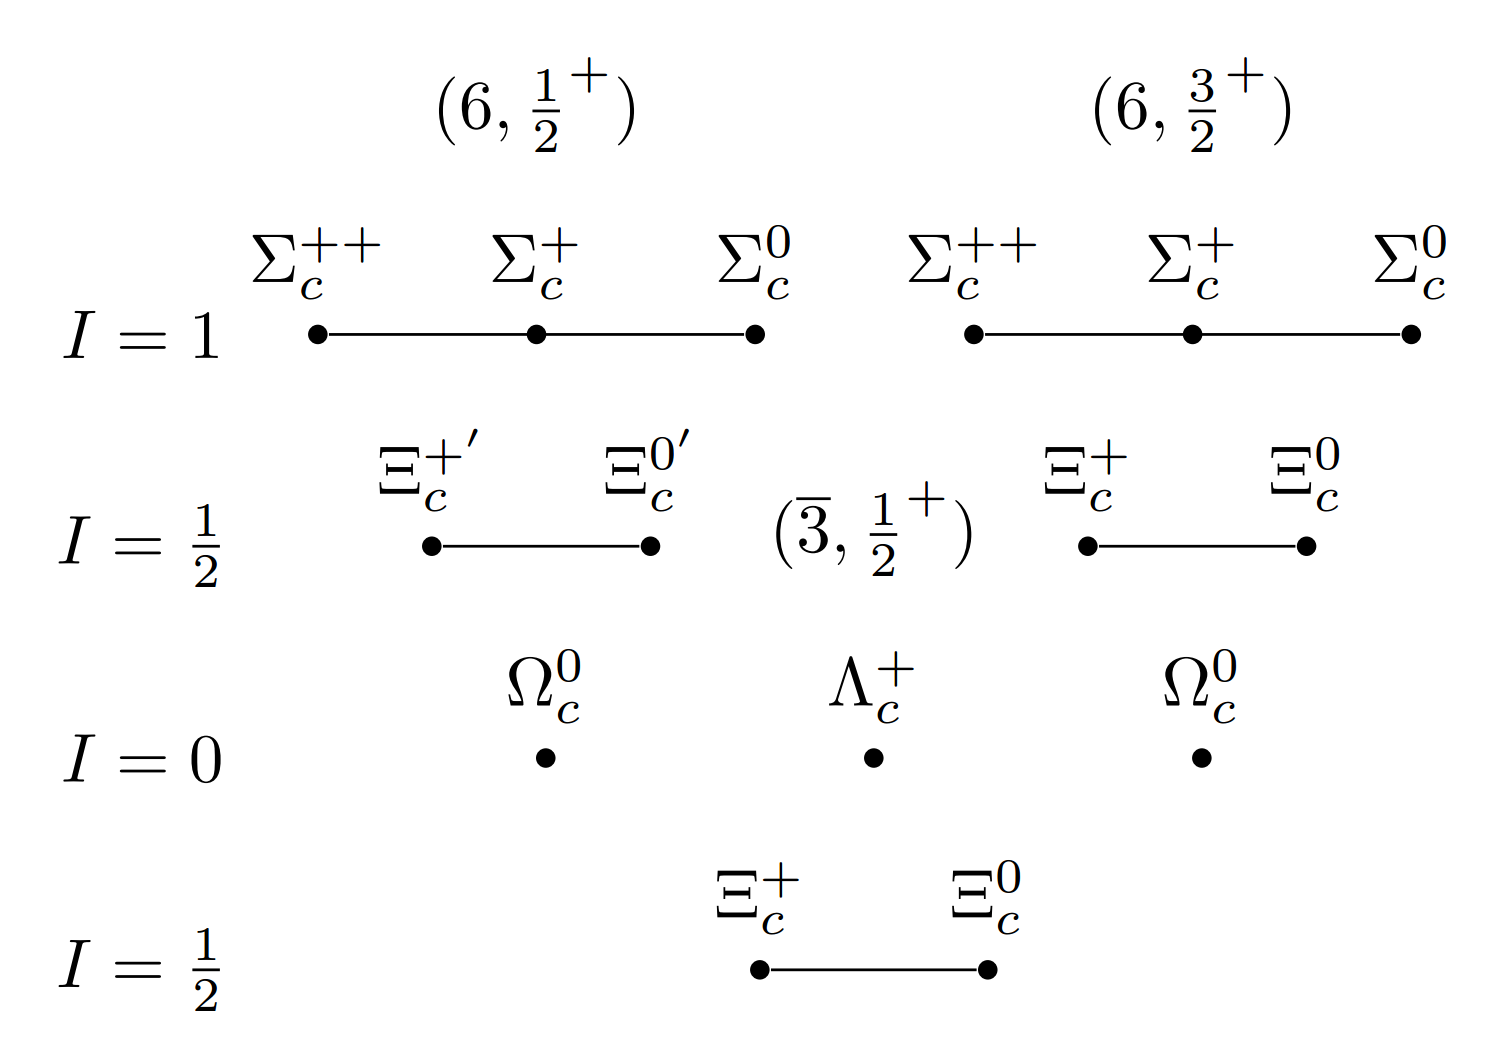
\includegraphics[scale=0.3]{multiplets.png}
		\caption{Một số đa tuyến điển hình (mỗi đường thẳng là một đa tuyến)}
	\end{figure}

\underline{Ví dụ}: đối với proton và neutron, ta có toán tử điện tích \( Q = I_{3} + \frac{1}{2} \) ( tổng phát phải là \( \frac{Q}{e} = I_{3} + \frac{1}{2} \) do \(I_{3}\) là đại lượng không thứ nguyên). Bểu diễn hạt thái của 2 hạt là:

	\begin{itemize}
		\item \( p = \left| \frac{1}{2} \enskip \frac{1}{2} \right\rangle\ \Rightarrow Q.p = 1.p \)
		\item \( n = \left| \frac{1}{2} \enskip - \frac{1}{2} \right\rangle\ \Rightarrow Q.n = 0.n \)
	\end{itemize}
	
Trong vật lý hạt cơ bản, các hardrons (Các hạt tham gia tương tác mạnh được cấu tạo bởi các quarks; phân biệt với lepton, các hạt không được cấu tạo bởi các quarks, chẳng hạn \(e\), \(\mu\), \(\tau\))	cũng được nhóm lại thành các đa tuyến của u(2). Đối với các hardrons, người ta định nghĩa số lượng tử gọi là siêu tích Y (hypercharge): tổng của số Baryon (B) và số lạ (S) 

\[ Y = B + S \]

Các hạt trong một đa tuyến được phân biệt bởi thành phần thứ 3 của isospin, thành phần thứ 3 của isospin được xác định bởi hệ thức Gell-mann \& Nishijima

\[ I_{3} = Q - \frac{Y}{2} = Q - \frac{B + S}{2} \Leftrightarrow Q = I_{3} + \frac{B + S}{2} \]

\section{Bảo toàn isospin}

Đối với các quá trình tương tác:

\underline{Tương tác mạnh}: isospin toàn phần \( I\) và \(I_{3}\) bảo toàn

\underline{Tương tác điện từ}: \(I\) không bảo toàn, \(I_{3}\) bảo toàn

\underline{Tương tác yếu}: \(I\) và \(I_{3}\) đều không bảo toàn

\underline{Ví dụ}: 

	\begin{align*}
		& \hspace*{0.3cm} \pi^{-} + p \hspace*{0.5cm} \longrightarrow \hspace*{0.7cm} \pi^{0} + n \\
		& initial \hspace*{0.1cm} state \hspace*{0.9cm} final \hspace*{0.1cm} state \\
		& \hspace*{-1.2cm} I \hspace*{0.4cm} 1 \otimes  \frac{1}{2} = \frac{3}{2} \oplus \frac{1}{2} \hspace*{1.1cm} 1 \otimes  \frac{1}{2} = \frac{3}{2} \oplus \frac{1}{2} \\
		& \hspace*{-1.2cm} I_{3} \hspace*{0.3cm} -1 + \frac{1}{2} = -\frac{1}{2} \hspace*{1.1cm} 0 - \frac{1}{2} = - \frac{1}{2}
	\end{align*}
	
Do \(I\) và \(I_{3}\) đều bảo toàn nên phản ứng trên xảy ra theo tương tác mạnh.

	\begin{align*}
		& \hspace*{0.3cm} d + d \hspace*{0.5cm} \longrightarrow \hspace*{0.7cm}^{4} He + \pi^{0} \\
		& initial \hspace*{0.1cm} state \hspace*{0.9cm} final \hspace*{0.1cm} state \\
		& \hspace*{-1.2cm} I \hspace*{1.2cm} 0 \otimes 0 = 0 \hspace*{1.3cm} 0 \otimes 1 = 1 \\
	\end{align*}

Phản ứng trên vi phạm bảo toàn isospin nhưng không xảy ra do không được ghi nhận trong thực nghiệm.

	\begin{align*}
		& \hspace*{0.3cm} \Sigma^{0} \hspace*{0.5cm} \longrightarrow \hspace*{0.7cm} \Lambda^{0} + \gamma \\
		& initial \hspace*{0.1cm} state \hspace*{0.9cm} final \hspace*{0.1cm} state \\
		& \hspace*{-1.2cm} I \hspace*{1.5cm} 1  \hspace*{3cm} 0 \\
		& \hspace*{-1.2cm} I_{3} \hspace*{1.4cm} 0 \hspace*{3cm} 0
	\end{align*}
	
Phân rã xảy ra theo tương tác điện từ.

	\begin{align*}
		& \hspace*{0.3cm} \Lambda^{0} \hspace*{0.5cm} \longrightarrow \hspace*{0.7cm} p + \pi^{-} \\
		& initial \hspace*{0.1cm} state \hspace*{0.9cm} final \hspace*{0.1cm} state \\
		& \hspace*{-1.2cm} I \hspace*{1.5cm} 0  \hspace*{1.8cm} 1 \otimes  \frac{1}{2} = \frac{3}{2} \oplus \frac{1}{2} \\
		& \hspace*{-1.2cm} I_{3} \hspace*{1.4cm} 0 \hspace*{1.8cm} -1 + \frac{1}{2} = -\frac{1}{2}
	\end{align*}
	
Phân rã xảy ra theo tương tác yếu.

\underline{Deuteron (d)}: pn bound state

\[ I = \frac{1}{2} \otimes \frac{1}{2} = 1 \oplus 0 \]

Nếu d có \( I = 1 \Rightarrow\) d là thành viên của tam tuyến (\(2I+1=3\)). Tam tuyến đó như sau:

	\begin{align*}
		& \left| 1 \enskip 1 \right\rangle\ = pp \\
		& \left| 1 \enskip 0 \right\rangle\ = \frac{1}{\sqrt{2}} (pn+np) \\
		& \left| 1 \enskip -1 \right\rangle\ = nn
	\end{align*}

Nếu d là \( \left| 1 \enskip 0 \right\rangle\ \) thì phải tồn tại trạng thái bound state của \(pp\) và \(nn\), nhưng do trong tự nhiên không tồn tại \(pp\) và \(nn\) nên \(I\) của isospin phải bằng 0.

Vậy d có isospin \( I = 0\), với \( p = \left| \frac{1}{2} \enskip \frac{1}{2} \right\rangle\ \), \( n = \left| \frac{1}{2} \enskip - \frac{1}{2} \right\rangle\ \)

\[ d = \frac{1}{\sqrt{2}} (pn-np) = \frac{1}{\sqrt{2}} \left( p \otimes n - n \otimes p \right) \]

Xét biểu diễn cơ bản của su(2): \( R_{f} \left( J_{i} \right) = \frac{1}{2} \sigma_{i} \)

	\begin{center}
		\( J_{1} \) = \( \begin{pmatrix}
			0 & 1/2 \\
			1/2 & 0 \\
		\end{pmatrix} \), \( J_{2} \) = \( \begin{pmatrix}
			0 & -i/2 \\
			i/2 & 0 \\
		\end{pmatrix} \), \( J_{3} \) = \(  \begin{pmatrix}
			1/2 & 0 \\
			0 & -1/2 \\
		\end{pmatrix} \)
	\end{center}
	
	\begin{center}
		\( J_{+} \) = \( J_{1} + i J_{2} \) = \( \begin{pmatrix}
			0 & 1 \\
			0 & 0 \\
		\end{pmatrix} \), \( J_{-} \) = \( J_{1} + i J_{2} \) = \( \begin{pmatrix}
			0 & 0 \\
			1 & 0 \\
		\end{pmatrix} \)
	\end{center}

Đặt \( p = \begin{pmatrix}
		1 \\ 0
	\end{pmatrix} \), và \( n = \begin{pmatrix}
		0 \\ 1
	\end{pmatrix} \) và 2 cơ sở của \( \mathbb{C}^{2} \)
	
	\begin{align*}
		& J_{3} p = \begin{pmatrix}
			1/2 & 0 \\
			0 & -1/2 \\
		\end{pmatrix} \begin{pmatrix}
			1 \\ 0
		\end{pmatrix} = \begin{pmatrix}
			1/2 \\ 0
		\end{pmatrix} = \frac{1}{2}.p \\
		& J_{+} p = \begin{pmatrix}
			0 & 1 \\
			0 & 0 \\
		\end{pmatrix} \begin{pmatrix}
			1 \\ 0
		\end{pmatrix} = \begin{pmatrix}
			0 \\ 0
		\end{pmatrix} = 0 \\
		& J_{-} p = \begin{pmatrix}
			0 & 0 \\
			1 & 0 \\
		\end{pmatrix} \begin{pmatrix}
			1 \\ 0
		\end{pmatrix} = \begin{pmatrix}
			0 \\ 1
		\end{pmatrix} = n \\
		& J_{3} n = \begin{pmatrix}
			1/2 & 0 \\
			0 & -1/2 \\
		\end{pmatrix} \begin{pmatrix}
			0 \\ 1
		\end{pmatrix} = \begin{pmatrix}
			0 \\ 1/2
		\end{pmatrix} = - \frac{1}{2}.n \\
		& J_{+} n = \begin{pmatrix}
			0 & 1 \\
			0 & 0 \\
		\end{pmatrix} \begin{pmatrix}
			0 \\ 1
		\end{pmatrix} = \begin{pmatrix}
			1 \\ 0
		\end{pmatrix} = p \\
		& J_{-} n = \begin{pmatrix}
			0 & 0 \\
			1 & 0 \\
		\end{pmatrix} \begin{pmatrix}
			0 \\ 1
		\end{pmatrix} = \begin{pmatrix}
			0 \\ 0
		\end{pmatrix} = 0
	\end{align*}
	
Rõ ràng:

	\begin{align*}
		& J_{3}p = \frac{1}{2}p \hspace*{3.8cm} J_{3}n = - \frac{1}{2}n \\
		& J_{+}p = 0 \hspace*{4cm} J_{+}n = p \\
		& J_{-}p = n \hspace*{4cm} J_{-}n = 0 \\
	\end{align*}
	
Xét iso-space: \( p = \left| \frac{1}{2} \enskip \frac{1}{2} \right\rangle\ \), \( n = \left| \frac{1}{2} \enskip - \frac{1}{2} \right\rangle\ \)

Nếu áp dụng các toán tử \( J_{3} \), \( J_{\pm} \) vào các trạng thái \( p \), \( n \) ta cũng có các kết quả trên, điển hình:
	\begin{align*}
		& J_{3}p = \frac{1}{2}.p + 0.n
		& J_{3}n = 0.p - \frac{1}{2}.p
	\end{align*}
	
\textbf{Lưu ý}: Không gian iso-space và không gian biểu diễn cơ bản của su(2) là 2 không gian khác nhau

\section{Biểu diễn bất khả quy hữu hạn chiều của su(3)}

Đại số Lie của su(3) có cơ sở gồm 8 (\(3^{2} - 1 = 8\)) ma trận cấp 3 có tính chất  hermitian và traceless

Ta chọn cơ sở là các ma trận Gell-mann:

	\begin{align*}
		& \lambda_{1} = \begin{pmatrix}
			0 & 1 & 0 \\
			1 & 0 & 0 \\
			0 & 0 & 0 \\
		\end{pmatrix}, \lambda_{2} = \begin{pmatrix}
			0 & -i & 0 \\
			i & 0 & 0 \\
			0 & 0 & 0 \\
		\end{pmatrix}, \lambda_{3} = \begin{pmatrix}
			1 & 0 & 0 \\
			0 & -1 & 0 \\
			0 & 0 & 0 \\
		\end{pmatrix} \\
		& \lambda_{4} =\begin{pmatrix}
			0 & 0 & 1 \\
			0 & 0 & 0 \\
			1 & 0 & 0 \\
		\end{pmatrix}, \lambda_{5} = \begin{pmatrix}
			0 & 0 & -i \\
			0 & 0 & 0 \\
			i & 0 & 0 \\
		\end{pmatrix} \\
		& \lambda_{6} = \begin{pmatrix}
			0 & 0 & 0 \\
			0 & 0 & 1 \\
			0 & 1 & 0 \\
		\end{pmatrix}, \lambda_{7} = \begin{pmatrix}
			0 & 0 & 0 \\
			0 & 0 & -i \\
			0 & i & 0 \\
		\end{pmatrix}, \lambda_{8} = \frac{2}{\sqrt{3}} \begin{pmatrix}
			1 & 0 & 0 \\
			0 & 1 & 0 \\
			0 & 0 & -2 \\
		\end{pmatrix} \\
	\end{align*}
		
	\begin{itemize}
		\item \( Tr \left( \lambda_{i} \lambda_{j} \right) = 2 \delta_{ij} \)
		\item \( \left[ \lambda_{i}, \lambda_{j} \right] = 2i \sum_{k} f_{ijk} \lambda_{k} = 2i f_{ijk} \lambda_{k} \)
		
		\[ \Rightarrow f_{ijk} = \frac{1}{4i} Tr \left( \left[ \lambda_{i}, \lambda_{j} \right] \lambda_{k} \right) \]
	\end{itemize}
		
	Đặt \( F_{i} = \frac{1}{2} \lambda_{i} \) với \( i = \overline{1, 8} \), ta có hệ thức giao hoán
	
	\[ \left[ F_{i}, F_{j} \right] = i f_{ijk} F_{k} \]
	
	Các tập sau đây xác định 3 biểu diễn của su(2)
	
	\begin{itemize}
		\item \( F_{1} \), \( F_{2} \), \( F_{3} \)
		\item \( F_{4} \), \( F_{5} \), \( \frac{1}{2} \left( \sqrt{3} F_{8} + F_{3} \right) \)
		\item \( F_{6} \), \( F_{7} \), \( \frac{1}{2} \left( \sqrt{3} F_{8} - F_{3} \right) \)
	\end{itemize}
	
	Bộ 3 các ma trận trên có hệ thức giao hoán tương tự su(2): \( \left[ \frac{\sigma_{i}}{2}, \frac{\sigma_{j}}{2} \right] = i \epsilon_{ijk} \frac{\sigma_{k}}{2} \)
	
	Cũng như su(2), ta đặt:
	
	\begin{itemize}
		\item \( I_{\pm} = F_{1} \pm i F_{2} \) \hspace*{1cm} \( I_{3} = F_{3} \) (isospin)
		\item \( V_{\pm} = F_{4} \pm i F_{5} \) \hspace*{1cm} \( V_{3} = \frac{1}{2} \left( \sqrt{3} F_{8} + F_{3} \right) \)
		\item \( U_{\pm} = F_{6} \pm i F_{7} \) \hspace*{1cm} \( U_{3} = \frac{1}{2} \left( \sqrt{3} F_{8} - F_{3} \right) \)
		\item \( Y = \frac{2}{\sqrt{3}} F_{8} \) (hypercharge)
	\end{itemize}
	
	Ta dùng ký hiệu \( F_{i} \) thay cho \( R(F_{i}) \) và hiểu \( F_{i} \) là biểu diễn của su(3)
	
	Ta có các hệ thức giao hoán cho biểu diễn của su(3):
	
	\begin{itemize}
		\item \( \left[ I_{3}, I_{\pm} \right] = \pm I_{\pm} \) \hspace*{0.9cm} \( \left[ I_{+}, I_{-} \right] = 2 I_{3} \)
		\item \( \left[ V_{3}, V_{\pm} \right] = \pm V_{\pm} \) \hspace*{0.8cm} \( \left[ V_{+}, V_{-} \right] = 2 V_{3} = \frac{3}{2} Y + I_{3} \)
		\item \( \left[ U_{3}, U_{\pm} \right] = \pm U_{\pm} \) \hspace*{0.7cm} \( \left[ U_{+}, U_{-} \right] = 2 U_{3} = \frac{3}{2} Y - I_{3} \)
		\item \( \left[ I_{3}, V_{\pm} \right] = \pm \frac{1}{2} V_{\pm} \) \hspace*{0.6cm} \( \left[ Y, V_{\pm} \right] = \pm V_{\pm} \)
		\item \( \left[ I_{3}, U_{\pm} \right] = \mp \frac{1}{2} V_{\pm} \) \hspace*{0.6cm} \( \left[ Y, U_{\pm} \right] = \pm U_{\pm} \)
		\item \( \left[ I_{3}, Y \right] = 0 \) \hspace*{1.6cm} \( \left[ Y, I_{\pm} \right] = 0 \)
		\item \( I_{\pm} \), \( V_{\pm} \), \( U_{\pm} \): toán tử tăng giảm
	\end{itemize}
	
	\textbf{Sơ đồ trọng (weight diagrams)}: 
	
	Gọi \( \left| \phi \right\rangle \) là trạng thái riêng của toán tử \( I_{3} \) và \( Y \) với trị riêng lần lượt là \( I_{3} \) và \( Y \)
	
	\( \widehat{I_{3}} \left| \phi \right\rangle = I_{3} \left| \phi \right\rangle \)
	
	\( \widehat{Y} \left| \phi \right\rangle = Y \left| \phi \right\rangle \)\\
	
	Từ các hệ thức giao hoán (ta bỏ dấu mũ vì tính thuận tiện):
	
	\begin{itemize}
		\item \( I_{3} \left( I_{\pm} \left| \phi \right\rangle \right) = \left( I_{3} \pm 1 \right) I_{\pm} \left| \phi \right\rangle \)
		\item \( Y \left( I_{\pm} \left| \phi \right\rangle \right) = Y I_{\pm} \left| \phi \right\rangle \)
		\item \( I_{3} \left( V_{\pm} \left| \phi \right\rangle \right) = \left( I_{3} \pm \frac{1}{2} \right) V_{\pm} \left| \phi \right\rangle \)
		\item \( Y \left( V_{\pm} \left| \phi \right\rangle \right) = \left( Y \pm 1 \right) V_{\pm} \left| \phi \right\rangle \)
		\item \( I_{3} \left( U_{\pm} \left| \phi \right\rangle \right) = \left( I_{3} \mp \frac{1}{2} \right) U_{\pm} \left| \phi \right\rangle \)
		\item \( Y \left( U_{\pm} \left| \phi \right\rangle \right) = \left( Y \pm 1 \right) U_{\pm} \left| \phi \right\rangle \)
	\end{itemize}
	
Điểm (\( I_{3}, Y \)) trong \( \mathbb{R}^{2} \) được gọi là trọng và \( \left| \phi \right\rangle \) là trạng thái có trọng (\( I_{3}, Y \)). Như vậy:
	
	\begin{itemize}
		\item \( I_{\pm} \left| \phi \right\rangle \) có trọng \( \left( I_{3}, Y \right) \pm \left( 1, 0 \right) \)
		\item \( V_{\pm} \left| \phi \right\rangle \) có trọng \( \left( I_{3}, Y \right) \pm \left( \frac{1}{2}, 0 \right) \)
		\item \( U_{\pm} \left| \phi \right\rangle \) có trọng \( \left( I_{3}, Y \right) \pm \left( - \frac{1}{2}, 0 \right) \)
	\end{itemize}

Từ các biểu diễn của su(2), ta biết rằng \( 2I_{3} \in \mathbb{Z} \), \( 2V_{3} \in \mathbb{Z} \), \( 2U_{3} \in \mathbb{Z} \) và \( 3Y \in \mathbb{Z} \)

Tập hợp các trọng (\( I_{3}, Y \)) được gọi là một sơ đồ trọng (weight diagram), với một biểu diễn hữu hạn chiều thì sơ đồ trọng chỉ có một số hữu hạn điểm. Tuy nhiên mỗi điểm trên một sơ đồ trọng có thể tương ứng với nhiều hơn một trạng thái riêng (multiplicity)

Gọi \( \left| \psi \right\rangle \) là trạng thái riêng của \( I_{3} \) và \( Y \) có trọng đại, thì khi đó \( \left| \psi \right\rangle \) thỏa:

\[ I_{+} \left| \psi \right\rangle = V_{+} \left| \psi \right\rangle = U_{+} \left| \psi \right\rangle = 0 \]

Áp dụng tất cả các tổ hợp có thể có của các toán tử giảm \( I_{-} \), \( V_{-} \), \( U_{-} \) trên trạng thái có trọng cực đại \( \left| \psi \right\rangle \) ta sẽ thu được biểu diễn bất khả quy hữu hạn chiều của su(3) (cũng chính là sơ đồ trọng)

	\begin{figure}[!htb]
		\centering
		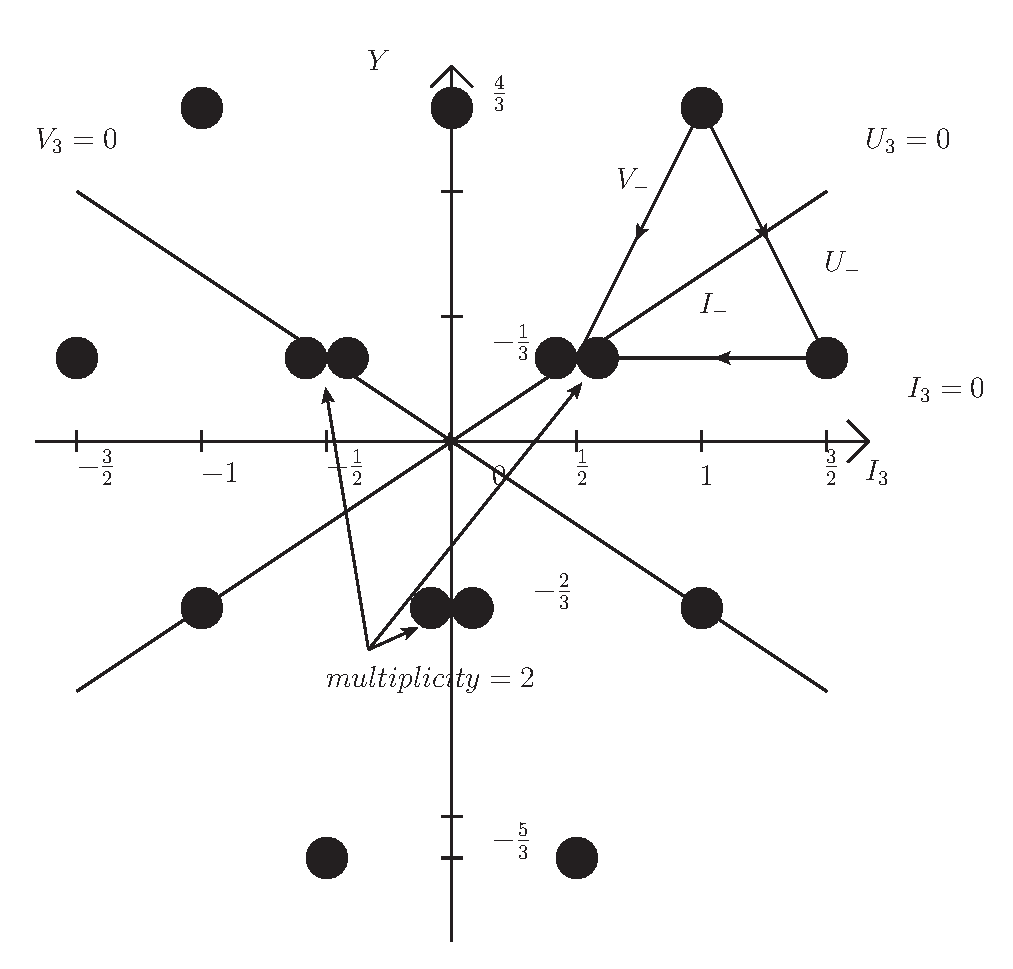
\includegraphics[scale=0.5]{diagram4.eps}
		\caption{Ví dụ về sơ đồ trọng}
	\end{figure}
	
\textbf{Nhận xét về sơ đồ trọng}:

Các trục \( I_{3} = 0 \), \( V_{3} = 0 \), \( U_{3} = 0 \) chứa các tâm đối xứng của các đa tuyến su(2). Từ đó suy ra sơ đồ trọng chỉ có thể có hình lục giác hoặc tam giác.

Lớp ngoài cùng của các sơ đồ trọng có multiplicity = 1, khi tiến vào bên trong thì multiplicity tăng 1 đơn vị cho đến khi gặp sơ đồ trọng tam giác đầu tiên thì số bội giữ nguyên không tahy đổi nữa cho dù có tiếp tục tiến vào lớp bên trong.

\section{Biểu diễn liên hợp phức}

Gọi R là biểu diễn của đại số Lie trong không gian phức V

	\begin{center}
		\( R \left( \left[ X, Y \right] \right) = \left[ R(X), R(Y) \right] \), \hspace*{0.5cm} \( X, Y \in g \) \\
		
		\( \Rightarrow R \left( \left[ X, Y \right] \right) \nu = R(X)R(Y) \nu - R(Y)R(X) \nu \), \hspace*{0.5cm} \( \nu \in V \) \\
		
		\( \Rightarrow R^{*} \left( \left[ X, Y \right] \right) \nu^{*} = R^{*}(X)R^{*}(Y) \nu^{*} - R^{*}(Y)R^{*}(X) \nu^{*} \) \\
		
		\( \Leftrightarrow R^{*} \left( \left[ X, Y \right] \right) = \left[ R^{*}(X), R^{*}(Y) \right] \)
	\end{center}
	
Đặt \( \bar{R}(x) = R^{*}(X) \) (*: liên hợp phức)	

\[ \Rightarrow \bar{R} \left( \left[ X, Y \right] \right) = \left[ \bar{R}(X), \bar{R}(Y) \right] \]

Do \( \bar{R} \) bảo toàn phép nhân Lie (đồng cấu đại số) nên  \( \bar{R} \) cũng là một biểu diễn của đại số Lie g trên V. Xét trường hợp đại số Lie su(n):\\

Giao hoán tử của ma trận phản hetmit: \( X_{i} \)

\[ \left[ X_{i}, X_{j} \right] = c_{ijk} X_{k} \]
\[ \Rightarrow \left[ R(X_{i}), R(X_{j}) \right] = c_{ijk} R(X_{k}) \]
\[ \Rightarrow\left[ R^{*}(X_{i}), R^{*}(X_{j}) \right] = c_{ijk} \\ R^{*}(X_{k}) \]

\hspace*{0.5cm} Nếu \( \bar{R}(X_{i}) = R^{*}(X_{i}) \) (quan trọng)

\[ \Rightarrow \bar{R}( \left[ X_{i}, X_{j} \right] ) = c_{ijk} \bar{R}(X_{k}) \]

Giao hoán tử của ma trận hermit: \( Y_{i} = i X_{i} \)

\[ \left[ Y_{i}, Y_{j} \right] = i c_{ijk} X_{k} \]
\[ \Rightarrow \left[ R(Y_{i}), R(Y_{j}) \right] = i c_{ijk} R(Y_{k}) \]
\[ \Rightarrow\left[ R^{*}(Y_{i}), R^{*}(Y_{j}) \right] = -i c_{ijk} \\ R^{*}(Y_{k}) \]
\[ \Rightarrow\left[ - R^{*}(Y_{i}), - R^{*}(Y_{j}) \right] = -i c_{ijk} \\ R^{*}(Y_{k}) \]

\hspace*{0.5cm} Nếu \( \bar{R}(Y_{i}) = - R^{*}(Y_{i}) \) (quan trọng)

\[ \Rightarrow \bar{R}( \left[ Y_{i}, Y_{j} \right] ) = i c_{ijk} \bar{R}(Y_{k}) \]

Vậy \( \bar{R} \) là một biểu diễn của su(n) và được gọi biểu diễn liên hợp phức của biểu diễn \( R \)

\underline{Ví dụ}: Biểu diễn liên hợp phức của biểu diễn cơ bản \( R_{f} \) của su(3) (\( R(F_{i}) = F_{i} \))

Do các ma trận \( F_{i} \) là các ma trận Hermit nên \( \bar{R}_{f}(F_{i}) = - F_{i} \)

	\begin{align*}
		\bar{I}_{+} & = \bar{R}_{f}(I_{+}) \\
		& = \bar{R}_{f}(F_{1} + i F_{2}) \\
		& = - F_{1}^{*} + (i F_{2})^{*} \\
		& = - F_{1}^{*} - i F_{2}^{*} \\
		& = - F_{1} + i F_{2} \\
		& = - I_{-}
	\end{align*}
	
Tương tự, ta có các biểu diễn sau:

	\begin{itemize}
		\item \( \bar{I}_{\pm} = - I_{\mp} \) \hspace*{1cm} \( \bar{I}_{3} = - I_{3} \)
		\item \( \bar{V}_{\pm} = - V_{\mp} \) \hspace*{0.8cm} \( \bar{V}_{3} = - V_{3} \)
		\item \( \bar{U}_{\pm} = - U_{\mp} \) \hspace*{0.8cm} \( \bar{U}_{3} = - U_{3} \)
	\end{itemize}
	
Ta thấy rằng các toán tử liên họp phức trên cũng thỏa mãn các hệ thức giao hoán giống như các toán tử	biểu diễn của chúng.

\section{Các biểu diễn số chiều thấp}

\hspace*{0.4cm} \textbf{Biểu diễn \( \mathbbm{1} \)}:

Trang thái \( \left| \psi \right\rangle \) có trọng cực đại (0, 0) 

\hspace{1cm} \( I_{3} \left| \psi \right\rangle = 0 \left| \psi \right\rangle \)

\hspace{1cm} \( Y \left| \psi \right\rangle = 0 \left| \psi \right\rangle \)

Nếu \( I_{\pm} \left| \psi \right\rangle = V_{\pm} \left| \psi \right\rangle = U_{\pm} \left| \psi \right\rangle = 0 \) thì không gian căng bởi  \( \left| \psi \right\rangle \neq 0\) là không gian 1 chiều

	\begin{figure}[!htb]
		\centering
		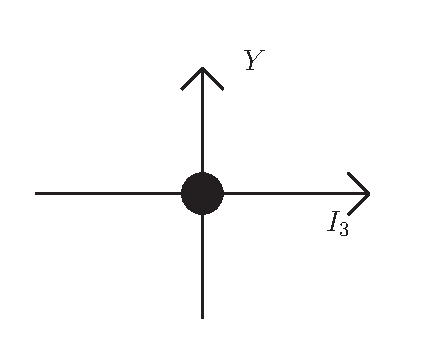
\includegraphics[scale=0.5]{diagram0.eps}
		\caption{sơ đồ trọng \( \mathbbm{1} \)}
	\end{figure}
		
\textbf{Biểu diễn \( \mathbb{3} \)}:
	
Xét biểu diễn \( R_{f} \)

	\begin{itemize}
		\item \( R_{f} ( I_{\pm} ) = I_{ \pm } \), \hspace*{0.5cm} \( R_{f} ( I_{3} ) = I_{ 3 } \)
		\item \( R_{f} ( V_{\pm} ) = V_{ \pm } \), \hspace*{0.4cm} \( R_{f} ( V_{3} ) = V_{ 3 } \)
		\item \( R_{f} ( U_{\pm} ) = U_{ \pm } \), \hspace*{0.4cm} \( R_{f} ( U_{3} ) = U_{ 3 } \)
		\item \( R_{f} ( Y ) = Y \)
	\end{itemize}
		
	\begin{center}
		\( I_{3} = \begin{pmatrix}
			1/2 & 0 & 0 \\
			0 & -1/2 & 0 \\
			0 & 0 & 0 \\
		\end{pmatrix} \), \hspace*{1cm} \( Y = \frac{1}{3} \begin{pmatrix}
			1 & 0 & 0 \\
			0 & 1 & 0 \\
			0 & 0 & -2 \\
		\end{pmatrix} \)
	\end{center}
	
Đặt: \( u \) = \( \begin{pmatrix}
			1 \\ 0 \\ 0
		\end{pmatrix} \), \( d \) = \( \begin{pmatrix}
			0 \\ 1 \\ 0
		\end{pmatrix} \), \( s \) = \( \begin{pmatrix}
			0 \\ 0 \\ 1
		\end{pmatrix} \)
		
Ta có:
	\begin{itemize}
		\item \( I_{3} u = \frac{1}{2} u \), \hspace*{0.7cm} \( Y u = \frac{1}{3}	u \)
		\item \( I_{3} d = - \frac{1}{2} d \), \hspace*{0.5cm} \( Y d = \frac{1}{3}	d \)
		\item \( I_{3} s = 0 \), \hspace*{1cm} \( Y s = - \frac{2}{3}	s \)
	\end{itemize}		
		
	\begin{center}
		\begin{tabular}{ |c|c|c|c|c|  }
			\hline
				\multicolumn{5}{|c|}{\( \mathbb{3} \)} \\
			\hline	
 				Trạng thái & Trọng & B & S & Q \\
 			\hline
 				\( u \) & \( \left( \frac{1}{2}, \frac{1}{3} \right) \) & \( \frac{1}{3} \) & 0 & \( \frac{2}{3} \) \\ 	
			\hline
 				\( d \) & \( \left( - \frac{1}{2}, \frac{1}{3} \right) \) & \( \frac{1}{3} \) & 0 & \( - \frac{1}{3} \) \\ 	
			\hline
				\( s \) & \( \left( 0, - \frac{2}{3} \right) \) & \( \frac{1}{3} \) & -1 & \( - \frac{1}{3} \) \\ 	
			\hline
	\end{tabular}
	\end{center}

Các quarks \( u \), \( d\), \( s\) đều có spin \( J = \frac{1}{2} \)

	\begin{figure}[!htb]
		\centering
		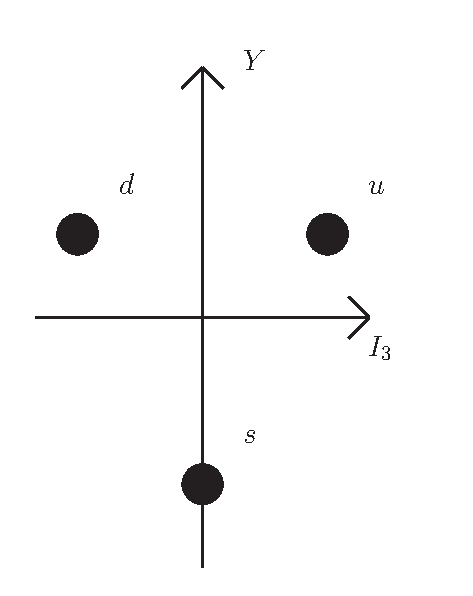
\includegraphics[scale=0.5]{diagram2.eps}
		\caption{sơ đồ trọng \( \mathbb{3} \)}
	\end{figure}
	
\textbf{Biểu diễn \( \bar{ \mathbb{3} } \)}:
	
Xét biểu diễn liên hợp phức của biểu diễn cơ bản:

	\begin{itemize}
		\item \( \bar{I}_{\pm} = - I_{ \mp } \), \hspace*{0.5cm} \( \bar{I}_{3} = - I_{ 3 } \)
		\item \( \bar{V}_{\pm} = - V_{ \mp } \), \hspace*{0.4cm} \( \bar{V}_{3} = - V_{ 3 } \)
		\item \( \bar{U}_{\pm} = - U_{ \mp } \), \hspace*{0.4cm} \( \bar{U}_{3} = - U_{ 3 } \)
		\item \( \bar{Y} = - Y \)
	\end{itemize}
	
Đặt: \( \bar{u} \) = \( \begin{pmatrix}
			1 \\ 0 \\ 0
		\end{pmatrix} \), \( \bar{d} \) = \( \begin{pmatrix}
			0 \\ 1 \\ 0
		\end{pmatrix} \), \( \bar{s} \) = \( \begin{pmatrix}
			0 \\ 0 \\ 1
		\end{pmatrix} \)
		
Ta có:

	\begin{itemize}
		\item \( \bar{I}_{3} \bar{u} = - \frac{1}{2} \bar{u} \), \hspace*{0.5cm} \( Y \bar{u} = - \frac{1}{3}	\bar{u} \)
		\item \( \bar{I}_{3} \bar{d} = \frac{1}{2} \bar{d} \), \hspace*{0.7cm} \( Y \bar{d} = - \frac{1}{3}	\bar{d} \)
		\item \( \bar{I}_{3} \bar{s} = 0 \), \hspace*{1cm} \( Y \bar{s} = \frac{2}{3}	\bar{s} \)
	\end{itemize}			
	
	\begin{center}
		\begin{tabular}{ |c|c|c|c|c|  }
			\hline
				\multicolumn{5}{|c|}{\( \bar{\mathbb{3}} \)} \\
			\hline	
 				Trạng thái & Trọng & B & S & Q \\
 			\hline
 				\( \bar{s} \) & \( \left( 0, \frac{2}{3} \right) \) & \( - \frac{1}{3} \) & 1 & \( \frac{1}{3} \) \\ 	
			\hline
 				\( \bar{d} \) & \( \left( \frac{1}{2}, - \frac{1}{3} \right) \) & \( - \frac{1}{3} \) & 0 & \( \frac{1}{3} \) \\ 	
			\hline
				\( \bar{u} \) & \( \left( - \frac{1}{2}, - \frac{1}{3} \right) \) & \( - \frac{1}{3} \) & 0 & \( - \frac{2}{3} \) \\ 	
			\hline
	\end{tabular}
	\end{center}

Các antiquarks (có điện tích trái dấu) \( \bar{u} \), \( \bar{d} \), \( \bar{s} \) đều có spin \( J = \frac{1}{2} \)

	\begin{figure}[!htb]
		\centering
		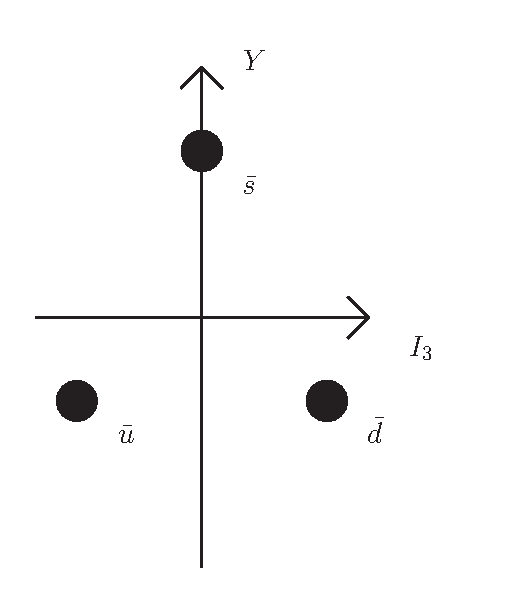
\includegraphics[scale=0.5]{diagram3.eps}
		\caption{sơ đồ trọng \( \bar{\mathbb{3}} \)}
	\end{figure}

\textbf{Biểu diễn \( \mathbb{8} \)}

Xét biểu diễn adjoint của đại số Lie su(3)

	\[ ad \left( \mathcal{A} \right) \left( \mathcal{B} \right) = \left[ \mathcal{A}, \mathcal{B} \right] \] 
	
Với \( \mathcal{A}, \mathcal{B} = I_{\pm}, I_{3}, V_{\pm}, V_{3}, U_{\pm}, U_{3} \).

Trọng của các trạng thái thu được từ các giao hoán tử sau: \( \left[ I_{3}, \mathcal{B} \right] \), \( \left[ Y, \mathcal{B} \right] \)

	\begin{center}
		\begin{tabular}{ |c|c|c|c| }
			\hline
 				Trạng thái &  \( \left[ I_{3}, \mathcal{B} \right] \) &  \( \left[ Y, \mathcal{B} \right] \) & Trọng \\
 			\hline
 				\( I_{3} \) & 0 & 0 & (0,0) \\
			\hline
 				\( Y \) & 0 & 0 & (0,0) \\
			\hline
				\( I_{+} \) & 1 & 0 & (1,0) \\	
			\hline
				\( I_{-} \) & -1 & 0 & (-1,0) \\	
			\hline
				\( V_{+} \) & \( \frac{1}{2} \) & 1 & (\( \frac{1}{2} \),1) \\	
			\hline
				\( V_{-} \) & \( - \frac{1}{2} \) & -1 & (\( - \frac{1}{2} \),-1) \\	
			\hline
				\( U_{+} \) & \( - \frac{1}{2} \) & 1 & (\( - \frac{1}{2} \),1) \\	
			\hline
				\( V_{-} \) & \( \frac{1}{2} \) & -1 & (\( \frac{1}{2} \),-1) \\	
			\hline
	\end{tabular}
	\end{center}	
	
	\begin{figure}[!htb]
		\centering
		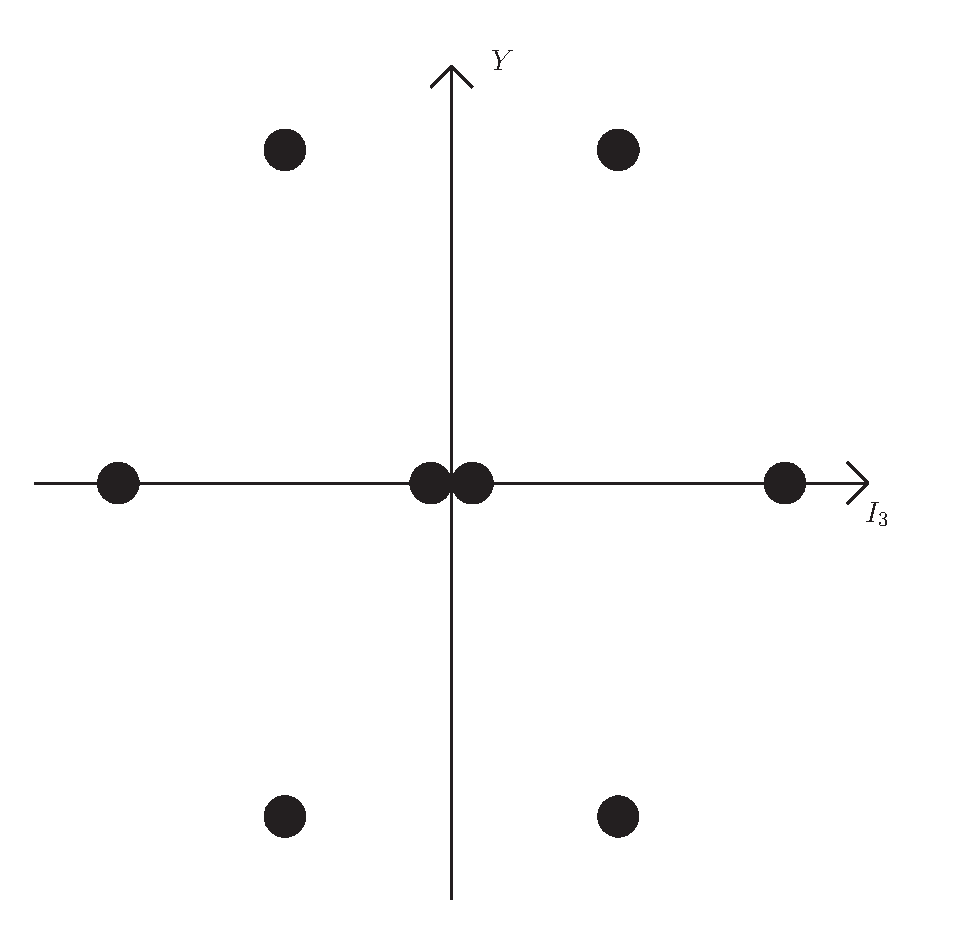
\includegraphics[scale=0.5]{diagram1.eps}
		\caption{sơ đồ trọng \(\mathbb{8}\)}
	\end{figure}	
	
Trong sơ đồ trọng \( \mathbb{8} \) thì chỉ có trọng (0,0) là có bậc 2, các trọng còn lại có bậc 1

\section{Biểu diễn tích tensor của su(3)}

Nhắc lại ở mục trước:

Cho \( R_{1} \) và \( R_{2} \) là biểu diễn của đại số Lie trên các không gian phức \( V_{1} \) và \( V_{2} \), \( \forall X \in g \), xét toán tử tuyến tính trên \( V_{1} \otimes V_{2} \) như sau:

\[ R(X) = R_{1}(X) \otimes \mathbbm{1} + \mathbbm{1} \otimes R_{2}(X) \]

Ta có \( R \left( \left[ X, Y \right] \right) = \left[ R(X), R(Y) \right] \); \( X, Y \in g \). Như vậy \( R(X) \) được xác định bởi biểu thức trên là một biểu diễn của đại số Lie g trên không gian tích tensor \( V_{1} \otimes V_{2} \) và được gọi là biểu diễn tích tensor của \( R_{1} \) và \( R_{2} \)

Tương tự ta có thể định nghĩa tích tensor của \( R_{1} \), \( R_{2} \) và \( R_{3} \) như sau:

\[ R(X) = R_{1}(X) \otimes \mathbbm{1} \otimes \mathbbm{1} + \mathbbm{1} \otimes R_{2}(X) \otimes \mathbbm{1} + \mathbbm{1} \otimes \mathbbm{1} \otimes R_{3}(X) \]

Nói chung biểu diễn tích tensor của \( R(X) \) là một biểu diễn khả quy và bây giờ ta sẽ phân tích thành tổng trực tiếp của những biểu diễn bất khả quy

\textbf{Phân tích biểu diễn tích tensor}:

Cho \( R_{1} \), \( R_{2} \) là 2 biểu diễn của su(3)

\hspace*{0.5cm} gọi \( \left| \phi_{1} \right\rangle \) là trạng thái riêng của \( R_{1}(I_{3}) \), \( R_{1}(Y) \) với trọng \( \left( I_{3}^{(1)}, Y^{(1)} \right) \)

\hspace*{1.1cm} \( \left| \phi_{2} \right\rangle \) là trạng thái riêng của \( R_{2}(I_{3}) \), \( R_{2}(Y) \) với trọng \( \left( I_{3}^{(2)}, Y^{(2)} \right) \)

Các toán tử tương ứng của biểu diễn tích tensor là:

	\begin{itemize}
		\item \( R(I_{3}) = R_{1}(I_{3}) \otimes \mathbbm{1} + \mathbbm{1} \otimes R_{2}(I_{3}) \)
		\item \( R(Y) = R_{1}(Y) \otimes \mathbbm{1} + \mathbbm{1} \otimes R_{2}(Y) \)
	\end{itemize}

Ta có :

	\begin{itemize}
		\item \( R(I_{3}) \left| \phi_{1} \right\rangle \otimes \left| \phi_{2} \right\rangle = \left( I_{3}^{(1)} + I_{3}^{(2)} \right) \left| \phi_{1} \right\rangle \otimes \left| \phi_{2} \right\rangle \)
		\item \( R(Y) \left| \phi_{1} \right\rangle \otimes \left| \phi_{2} \right\rangle = \left( Y^{(1)} + Y^{(2)} \right) \left| \phi_{1} \right\rangle \otimes \left| \phi_{2} \right\rangle \)
	\end{itemize}
	
Như vậy \( \left| \phi_{1} \right\rangle \otimes \left| \phi_{2} \right\rangle \) có trọng \( \left( I_{3}^{(1)} + I_{3}^{(2)}, Y^{(1)} + Y^{(2)} \right) \) =  \( \left( I_{3}^{(1)}, Y^{(1)} \right) \) + \( \left( I_{3}^{(2)}, Y^{(2)} \right) \)

Nghĩa là đối với biểu diễn tích tensor \( R \), các điểm trong sơ đồ trọng có được bằng cách cộng các cặp trọng như các vectơ trong mặt phẳng. Tuy nhiên mỗi điểm trong sơ đồ trọng của biểu diễn tích tensor có thể tương ứng với các trạng thái khác nhau trong tích \( V_{1} \otimes V_{2} \) (multiplicity).

Chọn trạng thái có trọng cực đại \( \left| \psi_{1} \right\rangle \otimes \left| \psi_{2} \right\rangle \) trong sơ đồ trọng \( R \) và áp dụng các toán tử giảm của tích tensor

	\begin{itemize}
		\item \( R(I_{\pm}) = R_{1}(I_{\pm}) \otimes \mathbbm{1} + \mathbbm{1} \otimes R_{2}(I_{\pm}) \)
		\item \( R(V_{\pm}) = R_{1}(V_{\pm}) \otimes \mathbbm{1} + \mathbbm{1} \otimes R_{2}(V_{\pm}) \)
		\item \( R(U_{\pm}) = R_{1}(U_{\pm}) \otimes \mathbbm{1} + \mathbbm{1} \otimes R_{2}(U_{\pm}) \)
	\end{itemize}

Khi đó ta sẽ thu được các trạng thái khác (ứng với các điểm trong sơ đồ trọng). Không gian căng bởi các trạng thái này là một không gian con bất biến \( W_{1} \) trong \( V_{1} \otimes V_{2} \), mà biểu diễn tích tnesor \( R \) trên không gian con \( W_{1} \) là biểu diễn bất khả quy.

Lấy ra các điểm trọng trong sơ đồ trọng tương ứng với các trạng thái cơ sở của \( W_{1} \). Lặp lại phương pháp này đối với các điểm còn lại trong sơ đồ trọng cho đến khi không còn điểm trọng nào trong sơ đồ trọng, cuối cùng không gian \( V_{1} \otimes V_{2} \) được phân tích thành tổng trực tiếp của các không gian con bất biến \( W_{j} \) mà biểu diễn tích tensor trên \( W_{j} \) là các biểu diễn bất khả quy.

	\[ V = V_{1} \otimes V_{2} = W_{1} \oplus W_{2} \oplus \cdots \oplus W_{m} \]
	
\textbf{Phân tích} \( \mathbb{3} \otimes \bar{\mathbb{3}} \)

Xét tích tensor \( \mathbb{3} \otimes \bar{\mathbb{3}} \): bằng cách cộng các trọng của \( \mathbb{3} \) và \( \bar{\mathbb{3}} \) ta thu được bảng các trạng thái và các trọng sau đây

	\begin{center}
		\begin{tabular}{ |c|c| }
			\hline
				\multicolumn{2}{|c|}{\( \mathbb{3} \otimes \bar{\mathbb{3}} \)} \\
			\hline	
 				Trạng thái & Trọng \\
 			\hline
 				\( u \otimes \bar{s} \) & \( \left( \frac{1}{2}, 1 \right) \) \\ 	
			\hline
 				\( u \otimes \bar{d} \) & \( \left( 1, 0 \right) \) \\ 	
			\hline
				\( d \otimes \bar{s} \) & \( \left( - \frac{1}{2}, 1 \right) \) \\ 	
			\hline
				\( u \otimes \bar{u} \), \( d \otimes \bar{d} \), \( s \otimes \bar{s} \) & \( \left( 0, 0 \right) \) \\ 	
			\hline
				\( d \otimes \bar{u} \) & \( \left( - 1, 0 \right) \) \\ 	
			\hline
				\( s \otimes \bar{u} \) & \( \left( - \frac{1}{2}, -1 \right) \) \\ 	
			\hline
				\( s \otimes \bar{d} \) & \( \left( \frac{1}{2}, - 1 \right) \) \\ 	
			\hline
	\end{tabular}
	\end{center}

	\begin{figure}[!htb]
		\centering
		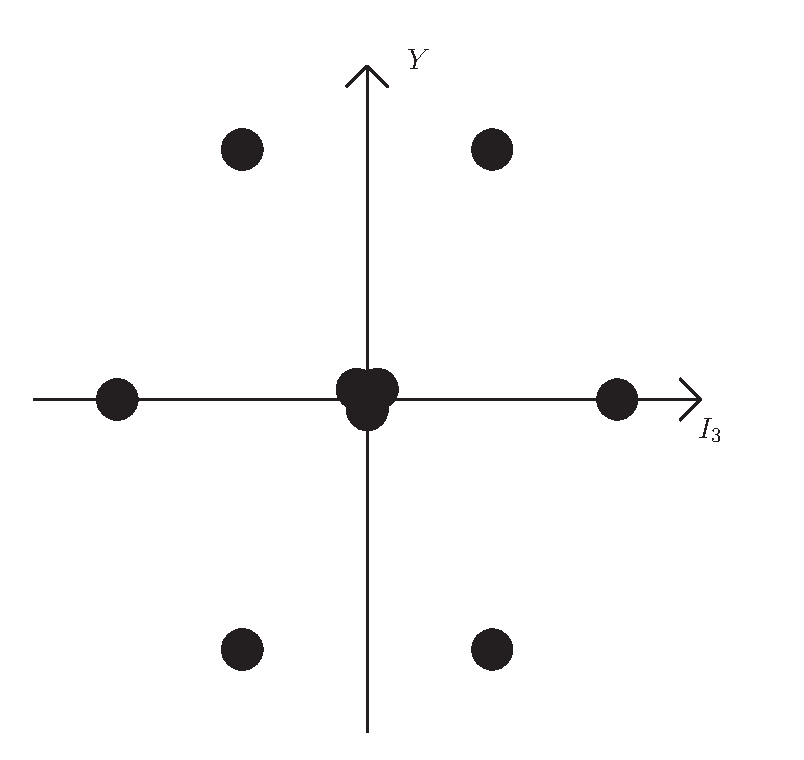
\includegraphics[scale=0.5]{diagram5.eps}
		\caption{sơ đồ trọng \( \mathbb{3} \otimes \bar{\mathbb{3}} \)}
	\end{figure}	
	
Các toán tử giảm trong không gian này:

	\begin{itemize}
		\item \( \mathcal{I}_{-} = I_{-} \otimes \mathbbm{1} + \mathbbm{1} \otimes \bar{I}_{-} \)
		\item \( \mathcal{V}_{-} = V_{-} \otimes \mathbbm{1} + \mathbbm{1} \otimes \bar{V}_{-} \)
		\item \( \mathcal{U}_{-} = U_{-} \otimes \mathbbm{1} + \mathbbm{1} \otimes \bar{U}_{-} \)
	\end{itemize}
	
Trạng thái có trọng cực đại \( u \otimes \bar{s} \), tác dụng tổ hợp các toán tử giảm ta thu được biểu diễn bất khả quy 8 chiều sau đây:

		\begin{center}
		\begin{tabu} to 0.8\textwidth { | X[c] | X[c] | }
			\hline
				\multicolumn{2}{|c|}{\( \mathbb{8} \) trong \( \mathbb{3} \otimes \bar{\mathbb{3}} \)} \\
			\hline	
 				Trạng thái & Trọng \\
 			\hline
 				\( u \otimes \bar{s} \) & \( \left( \frac{1}{2}, 1 \right) \) \\ 	
			\hline
 				\( u \otimes \bar{d} \) & \( \left( 1, 0 \right) \) \\ 	
			\hline
				\( d \otimes \bar{s} \) & \( \left( - \frac{1}{2}, 1 \right) \) \\ 	
			\hline
				\( \frac{1}{\sqrt{2}} \left( u \otimes \bar{u} - d \otimes \bar{d} \right) \) \hspace*{-0.4cm} \(  \frac{1}{\sqrt{6}} \left( u \otimes \bar{u} + d \otimes \bar{d} - 2 s \otimes \bar{s} \right) \)& \( \left( 0, 0 \right) \) \\ 	
			\hline
				\( d \otimes \bar{u} \) & \( \left( - 1, 0 \right) \) \\ 	
			\hline
				\( s \otimes \bar{u} \) & \( \left( - \frac{1}{2}, -1 \right) \) \\ 	
			\hline
				\( s \otimes \bar{d} \) & \( \left( \frac{1}{2}, - 1 \right) \) \\ 	
			\hline
		\end{tabu}
		\end{center}

	\begin{figure}[!htb]
		\centering
		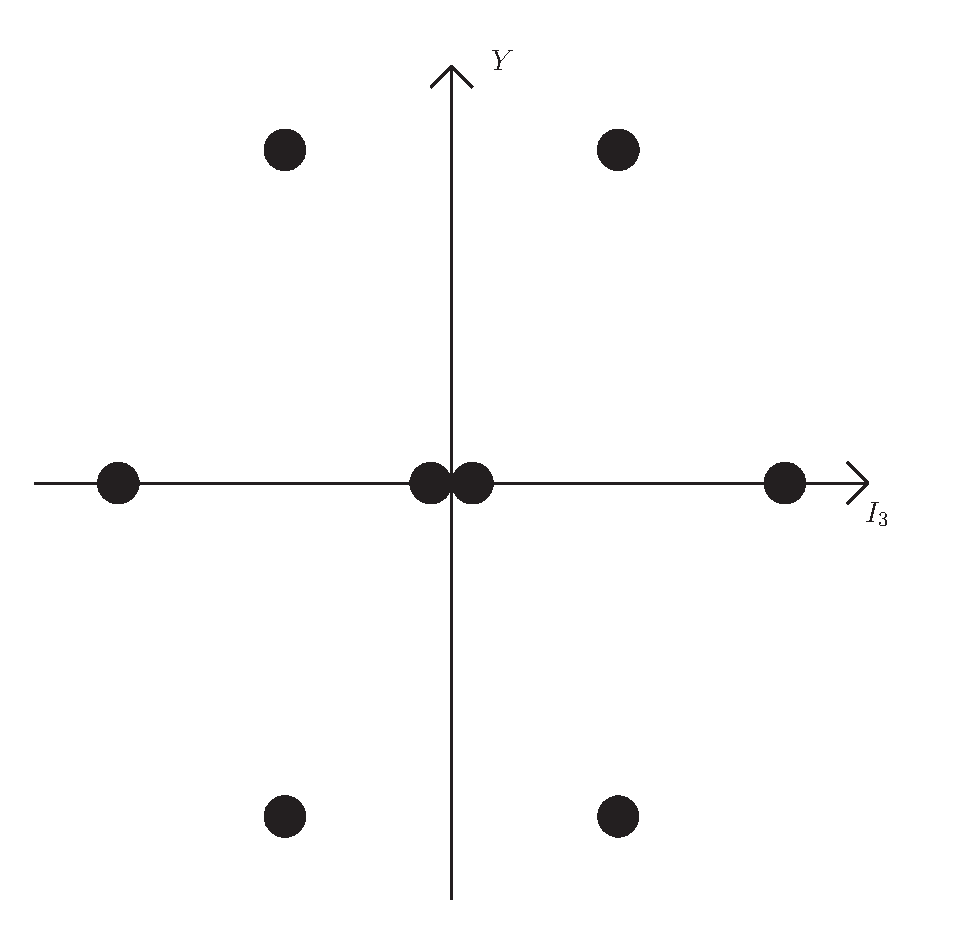
\includegraphics[scale=0.5]{diagram1.eps}
		\caption{sơ đồ trọng \(\mathbb{8}\)}
	\end{figure}

Sau khi lấy ra sơ đồ trọng \( \mathbb{8} \) ta có sơ đồ trọng còn lại, với trạng thái được ký hiệu: \( \mathbbm{1} = \frac{1}{\sqrt{3}} \left( u \otimes \bar{u} + d \otimes \bar{d} + s \otimes \bar{s} \right) \)

	\begin{figure}[!htb]
		\centering
		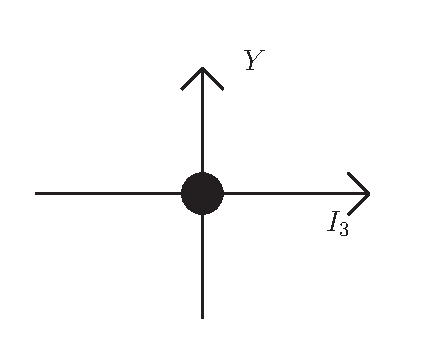
\includegraphics[scale=0.5]{diagram0.eps}
		\caption{sơ đồ trọng \( \mathbbm{1} \)}
	\end{figure}

Vậy \( \mathbb{3} \otimes \bar{\mathbb{3}} = \mathbb{8} \oplus \mathbb{1} \)

\underline{Bài tập}:

	\begin{itemize}
		\item chứng minh \( \left[ \mathcal{I}_{-}, \mathcal{U}_{-} \right] = - \mathcal{V}_{-} \)
		\item tính bảng \(\mathbb{8}\) trong \( \mathbb{3} \otimes \bar{\mathbb{3}} \) (gợi ý tính dựa vào giao hoán tử ở câu trên)
		\item tính bảng \(\mathbb{1}\) trong \( \mathbb{3} \otimes \bar{\mathbb{3}} \)
	\end{itemize}
	
\textbf{Bát tuyến giả vô hướng (Pseudoscalar octet - Meson octet)}: B = 0; J = 0

	\begin{figure}[!htb]
		\centering
		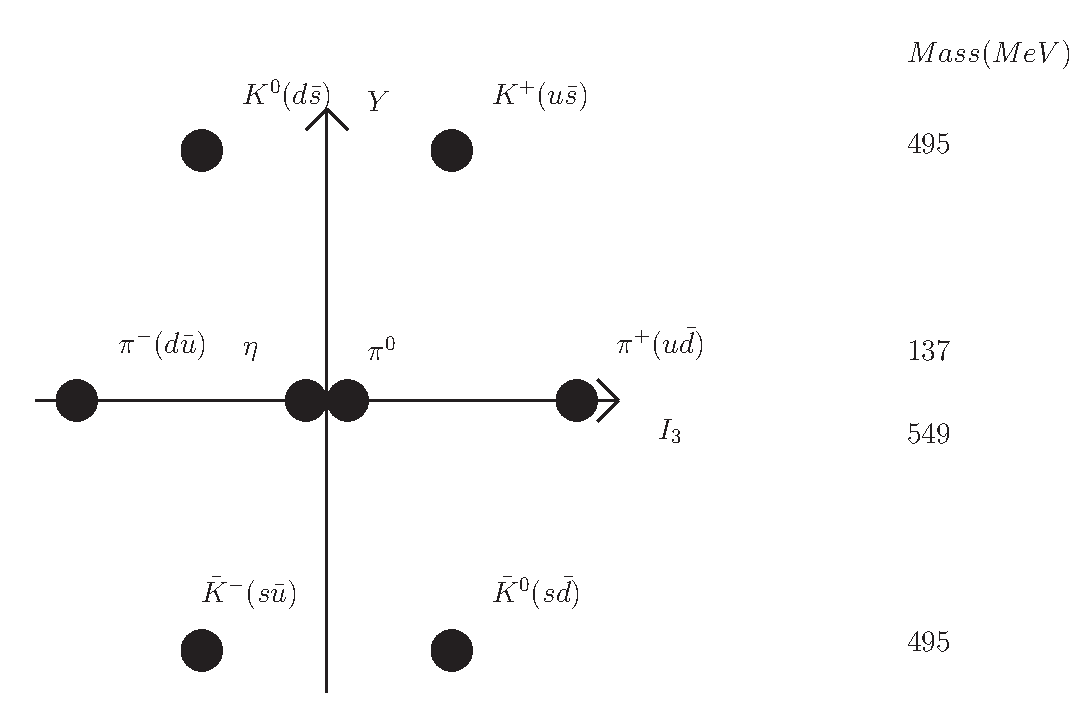
\includegraphics[scale=0.5]{diagram12.eps}
		\caption{Meson octet}
	\end{figure}
	
Với \( \pi^{0} = \frac{1}{\sqrt{2}} \left( u \otimes \bar{u} - d \otimes \bar{d} \right) \), \( \eta = \frac{1}{\sqrt{6}} \left( u \otimes \bar{u} + d \otimes \bar{d} - 2 s \otimes \bar{s} \right) \) \\

\textbf{Đơn tuyến meson}: \( \eta^{'} = \frac{1}{\sqrt{3}} \left( u \otimes \bar{u} + d \otimes \bar{d} + s \otimes \bar{s} \right) \) \\

\textbf{Phân tích} \( \mathbb{3} \otimes \mathbb{3} \otimes \mathbb{3} \)

Ta có bảng trọng và trạng thái sau:

	\begin{center}
		\begin{tabular}{ |c|c| }
			\hline
				\multicolumn{2}{|c|}{\( \mathbb{3} \otimes \mathbb{3} \otimes \mathbb{3} \)} \\
			\hline	
 				Trạng thái & Trọng \\
 			\hline
 				\( uuu \) & \( \left( \frac{3}{2}, 1 \right) \) \\ 	
			\hline
 				\( ddd \) & \( \left( - \frac{3}{2}, 1 \right) \) \\ 	
			\hline
				\( sss \) & \( \left( 0, - 2 \right) \) \\ 	
			\hline
				\( uud \), \( udu \), \( duu \) & \( \left( \frac{1}{2}, 1 \right) \) \\ 	
			\hline
				\( udd \), \( dud \), \( ddu \) & \( \left( - \frac{1}{2}, 1 \right) \) \\ 	
	
			\hline
				\( uus \), \( usu \), \( suu \) & \( \left( 1, 0 \right) \) \\ 	
			\hline
				\( uss \), \( sus \), \( ssu \) & \( \left( \frac{1}{2}, - 1 \right) \) \\ 	
			\hline
				\( dds \), \( dsd \), \( sdd \) & \( \left( - 1, 0 \right) \) \\ 	
			\hline
				\( dss \), \( sds \), \( ssd \) & \( \left( - \frac{1}{2}, - 1 \right) \) \\ 	
			\hline
				\( uds \), \( usd \), \( dus \), \( dsu \), \( sud \), \( sdu \) & \( \left( 0, 0 \right) \) \\ 	
			\hline
		\end{tabular}
	\end{center}

3 trạng thái đầu tiên có bội 1, các trạng thá tiếp theo có bội 3, trạng thái (0,0) có bội 6. Không gian của biểu diễn này là không gian 27 chiều.		

	\begin{figure}[!htb]
		\centering
		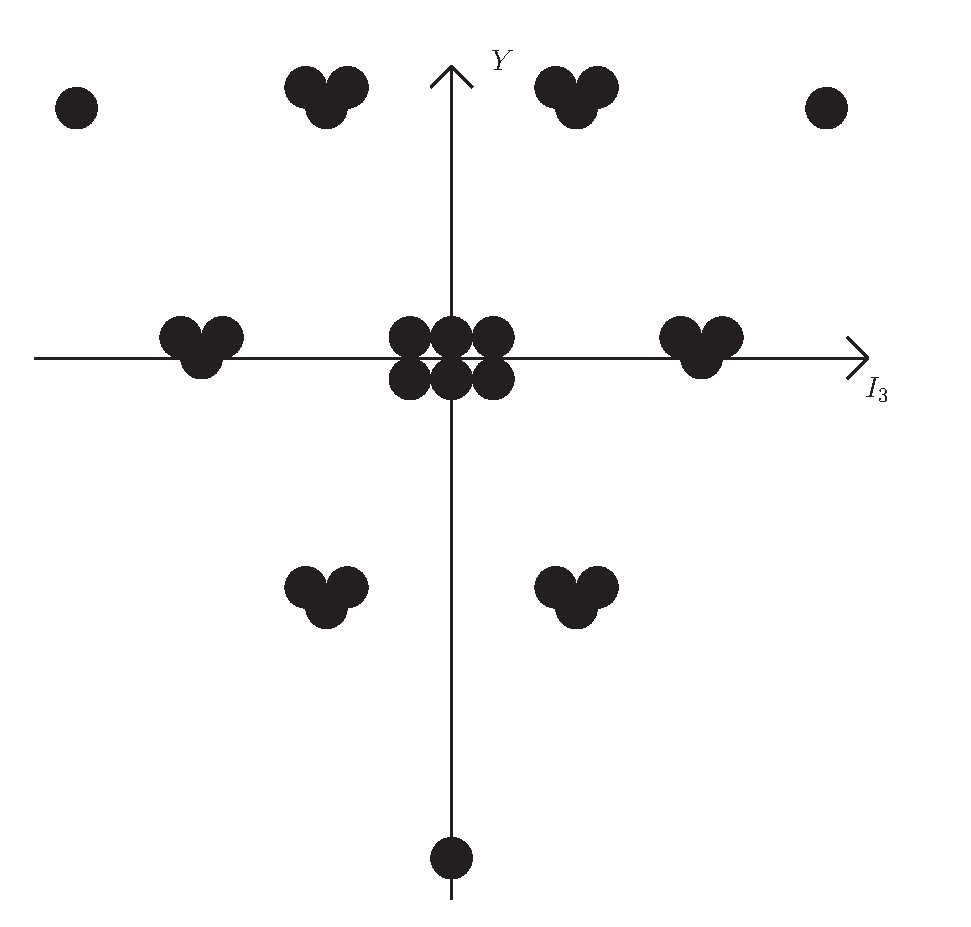
\includegraphics[scale=0.5]{diagram9.eps}
		\caption{sơ đồ trọng \( \mathbb{3} \otimes \mathbb{3} \otimes \mathbb{3} \)}
	\end{figure}

Các toán tử giảm trong không gian này:

	\begin{itemize}
		\item \( \mathcal{I}_{-} = I_{-} \otimes \mathbbm{1} \otimes \mathbbm{1} + \mathbbm{1} \otimes I_{-} \otimes \mathbbm{1} + \mathbbm{1} \otimes \mathbbm{1} \otimes I_{-} \)
		\item \( \mathcal{V}_{-} = V_{-} \otimes \mathbbm{1} \otimes \mathbbm{1} + \mathbbm{1} \otimes V_{-} \otimes \mathbbm{1} + \mathbbm{1} \otimes \mathbbm{1} \otimes V_{-} \)
		\item \( \mathcal{U}_{-} = U_{-} \otimes \mathbbm{1} \otimes \mathbbm{1} + \mathbbm{1} \otimes U_{-} \otimes \mathbbm{1} + \mathbbm{1} \otimes \mathbbm{1} \otimes U_{-} \)
	\end{itemize}	
	
Trạng thái có trọng cực dại là \( uuu \), áp dụng các toán tử giảm lên trạng thái này ta thu được biểu diễn bất khả quy 10 chiều:

	\begin{center}
		\begin{tabular}{ |c|c| }
			\hline
				\multicolumn{2}{|c|}{\( \mathbb{10} \) trong \( \mathbb{3} \otimes \mathbb{3} \otimes \mathbb{3} \)} \\
			\hline	
 				Trạng thái & Trọng \\
 			\hline
 				\( uuu \) & \( \left( \frac{3}{2}, 1 \right) \) \\ 	
			\hline
 				\( ddd \) & \( \left( - \frac{3}{2}, 1 \right) \) \\ 	
			\hline
				\( sss \) & \( \left( 0, - 2 \right) \) \\ 	
			\hline
				\( \frac{1}{\sqrt{3}} ( uud + udu + duu ) \) & \( \left( \frac{1}{2}, 1 \right) \) \\ 	
			\hline
				\( \frac{1}{\sqrt{3}} ( udd + dud + ddu ) \) & \( \left( - \frac{1}{2}, 1 \right) \) \\ 	
	
			\hline
				\( \frac{1}{\sqrt{3}} ( uus + usu + suu ) \) & \( \left( 1, 0 \right) \) \\ 	
			\hline
				\( \frac{1}{\sqrt{3}} ( uss + sus + ssu ) \) & \( \left( \frac{1}{2}, - 1 \right) \) \\ 	
			\hline
				\( \frac{1}{\sqrt{3}} ( dds + dsd + sdd ) \) & \( \left( - 1, 0 \right) \) \\ 	
			\hline
				\( \frac{1}{\sqrt{3}} ( dss + sds + ssd ) \) & \( \left( - \frac{1}{2}, - 1 \right) \) \\ 	
			\hline
				\( \frac{1}{\sqrt{6}} ( uds + usd + dus + dsu + sud + sdu ) \) & \( \left( 0, 0 \right) \) \\ 	
			\hline
		\end{tabular}
	\end{center}
	
	\begin{figure}[!htb]
		\centering
		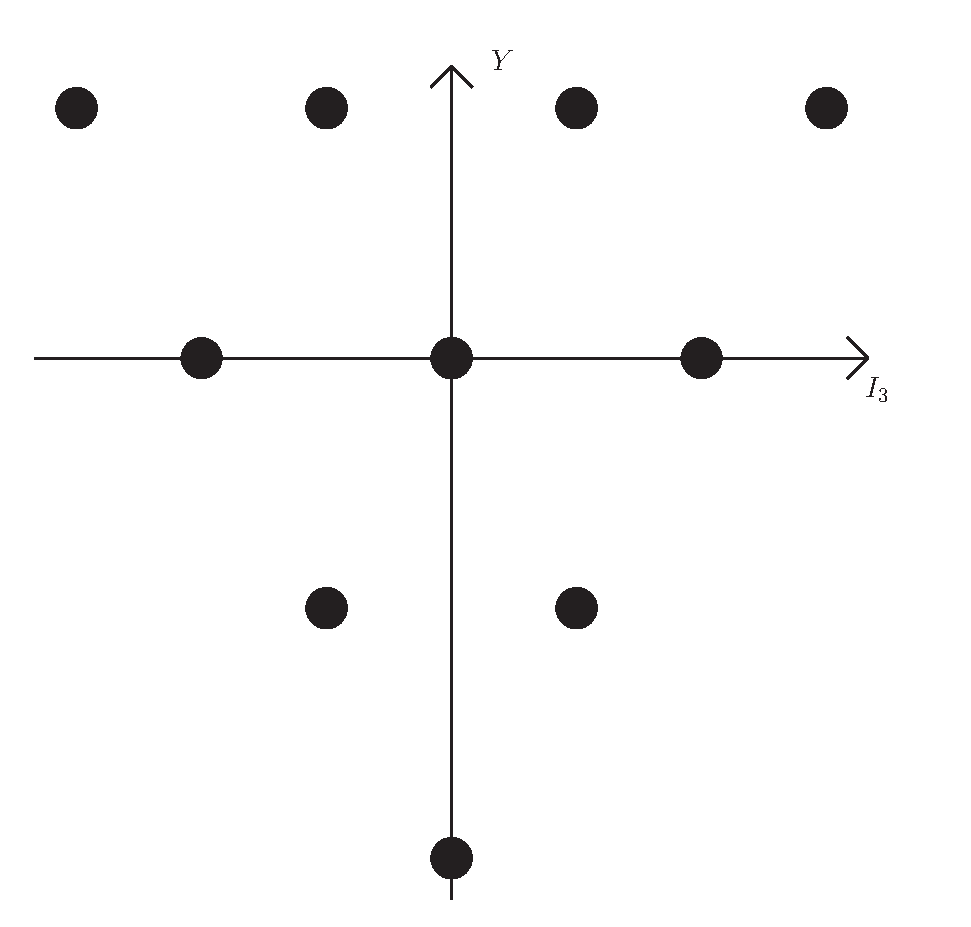
\includegraphics[scale=0.4]{diagram8.eps}
		\caption{sơ đồ trọng \( \mathbb{10} \)}
	\end{figure}	

Lấy ra không gian con 10 chiều này, không gian con còn lại trong không gian tích tensor là 17 chiều, sơ đồ trọng còn lại là:

	\begin{figure}[!htb]
		\centering
		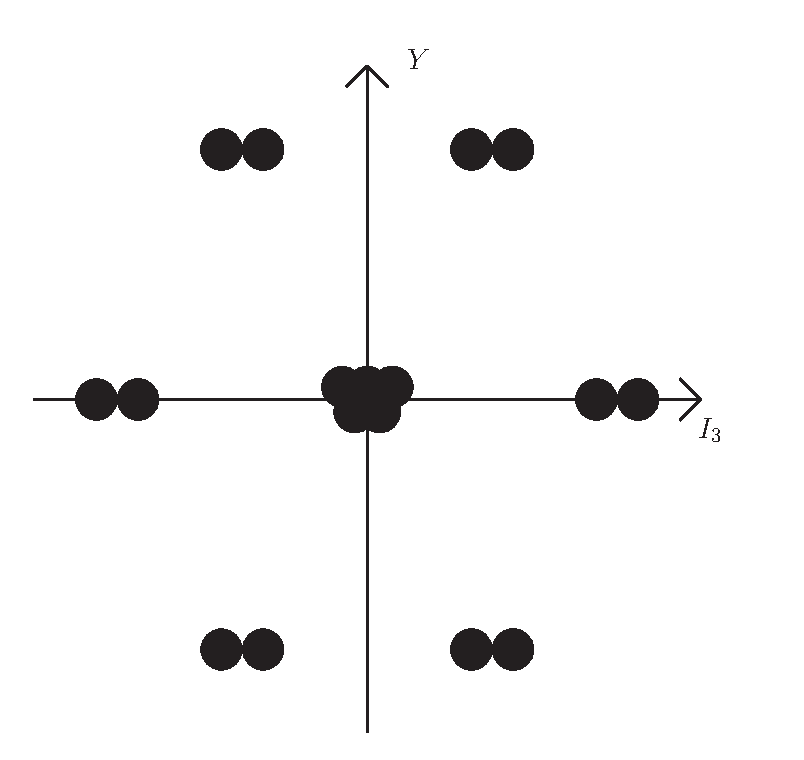
\includegraphics[scale=0.5]{diagram7.eps}
		\caption{sơ đồ trọng còn lại}
	\end{figure}	

Lúc này trọng cực đại là \( \left( \frac{1}{2}, 1 \right) \) (tuy nhiên trọng cực này không pah3i là duy nhất do đây là biểu diễn khả quy): có 2 trạng thái trực giao tương ứng với trọng này:

	\begin{itemize}
		\item \( \left| \psi_{1} \right\rangle = \frac{1}{\sqrt{2}} \left( duu - udu \right) \)
		\item \( \left| \psi_{2} \right\rangle = \frac{1}{\sqrt{6}} \left( duu + udu - 2 uud \right) \)
	\end{itemize}
	
	\begin{center}
		\begin{tabu} to 1\textwidth { | X[c] | X[c] | }
			\hline
				\multicolumn{2}{|c|}{\( \mathbb{8} \) trong \( \mathbb{3} \otimes \mathbb{3} \otimes \mathbb{3}  \)} \\
			\hline	
 				Trạng thái & Trọng \\
 			\hline
 				\( \frac{1}{\sqrt{2}} \left( duu - udu \right) \) & \( \left( \frac{1}{2}, 1 \right) \) \\ 	
			\hline
 				\( \frac{1}{\sqrt{2}} \left( suu - usu \right) \) & \( \left( 1, 0 \right) \) \\ 	
			\hline
				\( \frac{1}{\sqrt{2}} \left( dud - udd \right) \) & \( \left( - \frac{1}{2}, 1 \right) \) \\ 	
			\hline
				\( \frac{1}{2} \left( dsu + dus  - sdu - uds \right) \) \hspace*{-0.1cm} \( \frac{1}{2} \left( sdu + sud  - dsu - usd \right) \)& \( \left( 0, 0 \right) \) \\ 	
			\hline
				\( \frac{1}{\sqrt{2}} \left( dsd - sdd \right) \) & \( \left( - 1, 0 \right) \) \\ 	
			\hline
				\( \frac{1}{\sqrt{2}} \left( dss - sds \right) \) & \( \left( - \frac{1}{2}, -1 \right) \) \\ 	
			\hline
				\( \frac{1}{\sqrt{2}} \left( sus - uss \right) \) & \( \left( \frac{1}{2}, - 1 \right) \) \\ 	
			\hline
		\end{tabu}
		\end{center}

	\begin{center}
		\begin{tabu} to 1.3\textwidth { | X[c] | X[c] | }
			\hline
				\multicolumn{2}{|c|}{\( \mathbb{8} \) trong \( \mathbb{3} \otimes \mathbb{3} \otimes \mathbb{3}  \)} \\
			\hline	
 				Trạng thái & Trọng \\
 			\hline
 				\(  \frac{1}{\sqrt{6}} \left( duu + udu - 2 uud \right) \) & \( \left( \frac{1}{2}, 1 \right) \) \\ 	
			\hline
 				\(  \frac{1}{\sqrt{6}} \left( suu + usu - 2 uus \right) \) & \( \left( 1, 0 \right) \) \\ 	
			\hline
				\(  \frac{1}{\sqrt{6}} \left( 2 ddu - dud - udd \right) \) & \( \left( - \frac{1}{2}, 1 \right) \) \\ 	
			\hline
				\(  \frac{1}{2 \sqrt{3}} \left( dsu + dus + sdu + uds - 2 sud - 2 usd \right) \) \hspace*{-0.1cm} \(  \frac{1}{2 \sqrt{3}} \left( sdu + sud + dsu + usd - 2 dus - 2uds \right) \) & \( \left( 0, 0 \right) \) \\ 	
			\hline
				\(  \frac{1}{\sqrt{6}} \left( 2 dds - dsd - sdd \right) \) & \( \left( - 1, 0 \right) \) \\ 	
			\hline
				\(  \frac{1}{\sqrt{6}} \left( sds + dss - 2 ssd \right) \) & \( \left( - \frac{1}{2}, -1 \right) \) \\ 	
			\hline
				\(  \frac{1}{\sqrt{6}} \left( 2 ssu - sus -  uss \right) \) & \( \left( \frac{1}{2}, - 1 \right) \) \\ 	
			\hline
		\end{tabu}
		\end{center}	
	
Sau khi lấy ra 2 không gian 8 chiều này, không gian còn lại là 1 chiều, sơ đồ trọng còn lại là:	
	
	\begin{figure}[!htb]
		\centering
		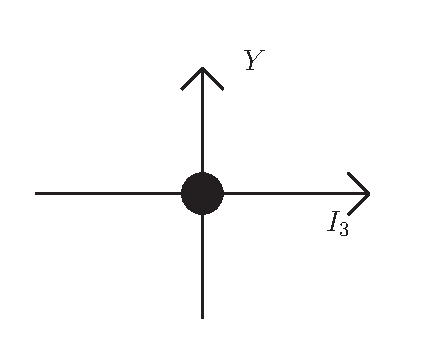
\includegraphics[scale=0.5]{diagram0.eps}
		\caption{sơ đồ trọng \( \mathbbm{1} \) trong trong \( \mathbb{3} \otimes \mathbb{3} \otimes \mathbb{3}  \)}
	\end{figure}	
	
Ứng với trạng thái: \(  \frac{1}{\sqrt{6}} \left( uds + sud + dsu - sdu - dus - usd \right) \)

\underline{Bài tập}:

	\begin{itemize}
		\item Tính \( \mathbb{10} \) trong \( \mathbb{3} \otimes \mathbb{3} \otimes \mathbb{3}  \)
		\item Tính 2 bảng \( \mathbbm{8} \) trong \( \mathbb{3} \otimes \mathbb{3} \otimes \mathbb{3}  \) và 2 trạng thái có trọng cực dại tương ứng với chúng
		\item Tính \( \mathbbm{1} \) trong \( \mathbb{3} \otimes \mathbb{3} \otimes \mathbb{3}  \)
	\end{itemize}
	
\textbf{Thập tuyến baryon} B = 1, J = \( \frac{3}{2} \)

	\begin{figure}[!htb]
		\centering
		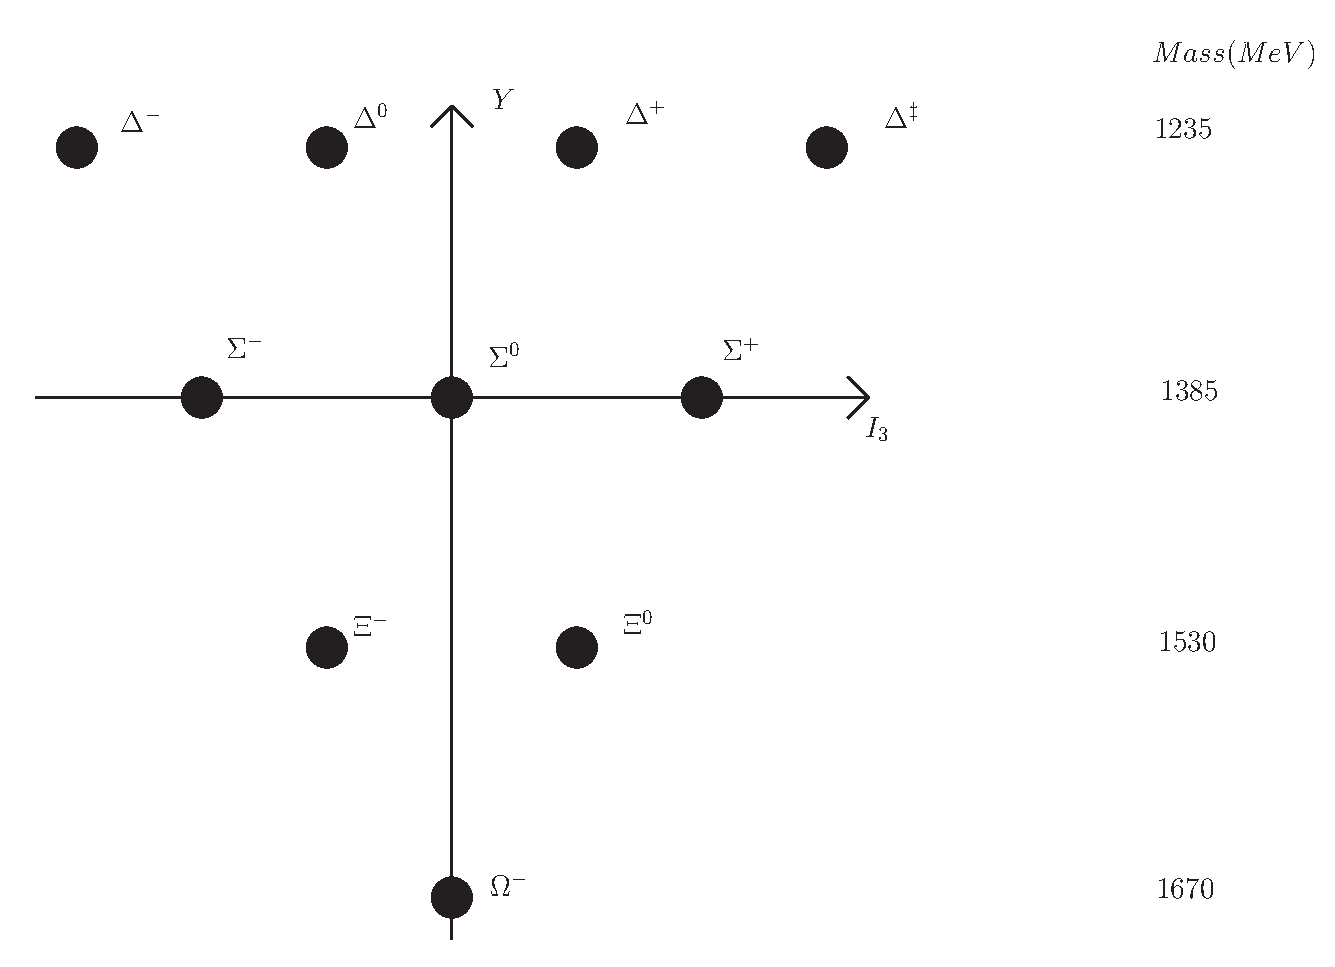
\includegraphics[scale=0.5]{diagram10.eps}
		\caption{Baryon decuptet}
	\end{figure}
	
\textbf{Bát tuyến baryon} B = 1, J = \( \frac{1}{2} \) (ứng với trọng cực đại \( \left| \psi_{1} \right\rangle \))

	\begin{figure}[!htb]
		\centering
		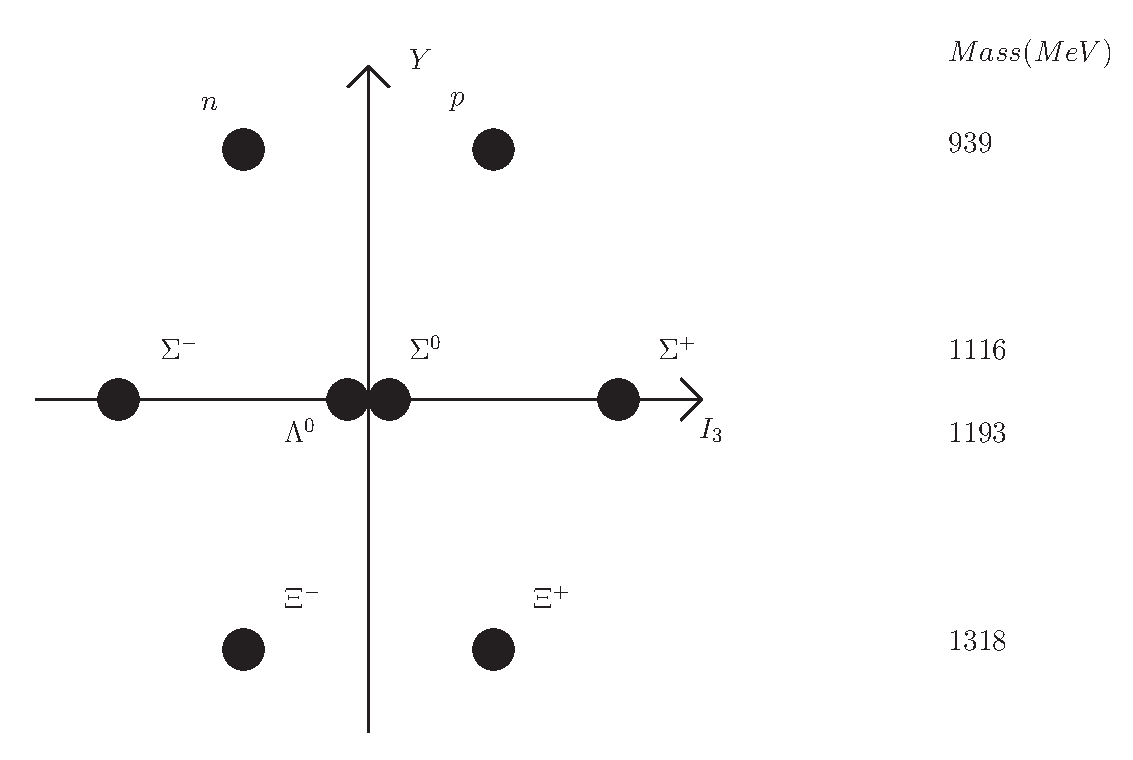
\includegraphics[scale=0.5]{diagram11.eps}
		\caption{Baryon octet}
	\end{figure}	
	
\textbf{Đơn tuyến baryon} B = 1, J = \( \frac{1}{2} \): \( \Lambda^{0} \)
	
\end{document}